\documentclass[a4paper,UKenglish,cleveref, autoref, thm-restate]{lipics-v2021}
%See lipics-v2021-authors-guidelines.pdf for further information.
%for A4 paper format use option "a4paper", for US-letter use option "letterpaper"
%for british hyphenation rules use option "UKenglish", for american hyphenation rules use option "USenglish"
%for section-numbered lemmas etc., use "numberwithinsect"
%for enabling cleveref support, use "cleveref"
%for enabling autoref support, use "autoref"
%for anonymousing the authors (e.g. for double-blind review), add "anonymous"
%for enabling thm-restate support, use "thm-restate"
%for enabling a two-column layout for the author/affilation part (only applicable for > 6 authors), use "authorcolumns"

\usepackage{todonotes}
\usepackage{numprint}
\npstyleenglish
\usepackage{placeins}

\usepackage[ruled,vlined,linesnumbered,norelsize]{algorithm2e}
\DontPrintSemicolon
\def\NlSty#1{\textnormal{\fontsize{8}{10}\selectfont{}#1}}
\SetKwSty{texttt}
\SetCommentSty{emph}
\def\algorithmautorefname{Algorithm}

\listfiles

%\graphicspath{{./graphics/}}%helpful if your graphic files are in another directory

\bibliographystyle{plainurl}% the mandatory bibstyle

\title{Targeted Branching for the Maximum Independent Set Problem} %TODO Please add

\titlerunning{Targeted Branching for the MIS Problem} %TODO optional, please use if title is longer than one line

% \author{John Q. Public}{Dummy University Computing Laboratory, [optional: Address], Country \and My second affiliation, Country \and \url{http://www.myhomepage.edu} }{johnqpublic@dummyuni.org}{https://orcid.org/0000-0002-1825-0097}{(Optional) author-specific funding acknowledgements}%TODO mandatory, please use full name; only 1 author per \author macro; first two parameters are mandatory, other parameters can be empty. Please provide at least the name of the affiliation and the country. The full address is optional

\author{Demian Hespe}{Karlsruhe Institute of Technology, Institute for
  Theoretical Informatics, Germany}{hespe@kit.edu}{https://orcid.org/0000-0001-6232-2951}{}

\author{Sebastian Lamm}{Karlsruhe Institute of Technology, Institute for
  Theoretical Informatics, Germany}{lamm@kit.edu}{}{\todo{Add funding}}

\author{Christian Schorr}{Karlsruhe Institute of Technology, Institute for
  Theoretical Informatics, Germany}{christian.schorr@student.kit.edu}{}{}

\authorrunning{D. Hespe and S. Lamm and C. Schorr} %TODO mandatory. First: Use abbreviated first/middle names. Second (only in severe cases): Use first author plus 'et al.'

\Copyright{Demian Hespe and Sebastian Lamm and Christian Schorr} %TODO mandatory, please use full first names. LIPIcs license is "CC-BY";  http://creativecommons.org/licenses/by/3.0/
\begin{CCSXML}
  <ccs2012>
  <concept>
  <concept_id>10002950.10003624.10003633.10010917</concept_id>
  <concept_desc>Mathematics of computing~Graph algorithms</concept_desc>
  <concept_significance>500</concept_significance>
  </concept>
  <concept>
  <concept_id>10003752.10003809.10011254.10011256</concept_id>
  <concept_desc>Theory of computation~Branch-and-bound</concept_desc>
  <concept_significance>500</concept_significance>
  </concept>
  <concept>
  <concept_id>10002950.10003624.10003625.10003630</concept_id>
  <concept_desc>Mathematics of computing~Combinatorial optimization</concept_desc>
  <concept_significance>500</concept_significance>
  </concept>
  </ccs2012>
\end{CCSXML}

\ccsdesc[500]{Mathematics of computing~Graph algorithms}
\ccsdesc[500]{Theory of computation~Branch-and-bound}
\ccsdesc[500]{Mathematics of computing~Combinatorial optimization}
% \ccsdesc[100]{\textcolor{red}{Replace ccsdesc macro with valid oll
% ne}} %TODO mandatory: Please choose ACM 2012 classifications from https://dl.acm.org/ccs/ccs_flat.cfm 

\keywords{Graphs, Combinatorial Optimization, Independent Set, Vertex Cover,
  Clique, Branch-and-Reduce, Branch-and-Bound, Kernelization}%TODO mandatory; please add comma-separated list of keywords

\category{} %optional, e.g. invited paper

\relatedversion{} %optional, e.g. full version hosted on arXiv, HAL, or other respository/website
%\relatedversiondetails[linktext={opt. text shown instead of the URL}, cite=DBLP:books/mk/GrayR93]{Classification (e.g. Full Version, Extended Version, Previous Version}{URL to related version} %linktext and cite are optional

%\supplement{}%optional, e.g. related research data, source code, ... hosted on a repository like zenodo, figshare, GitHub, ...
%\supplementdetails[linktext={opt. text shown instead of the URL}, cite=DBLP:books/mk/GrayR93, subcategory={Description, Subcategory}, swhid={Software Heritage Identifier}]{General Classification (e.g. Software, Dataset, Model, ...)}{URL to related version} %linktext, cite, and subcategory are optional

%\funding{(Optional) general funding statement \dots}%optional, to capture a funding statement, which applies to all authors. Please enter author specific funding statements as fifth argument of the \author macro.

\acknowledgements{}%optional

%\nolinenumbers %uncomment to disable line numbering

% \hideLIPIcs  %uncomment to remove references to LIPIcs series (logo, DOI, ...), e.g. when preparing a pre-final version to be uploaded to arXiv or another public repository

%Editor-only macros:: begin (do not touch as author)%%%%%%%%%%%%%%%%%%%%%%%%%%%%%%%%%%
\EventEditors{John Q. Open and Joan R. Access}
\EventNoEds{2}
\EventLongTitle{42nd Conference on Very Important Topics (CVIT 2016)}
\EventShortTitle{CVIT 2016}
\EventAcronym{CVIT}
\EventYear{2016}
\EventDate{December 24--27, 2016}
\EventLocation{Little Whinging, United Kingdom}
\EventLogo{}
\SeriesVolume{42}
\ArticleNo{23}
%%%%%%%%%%%%%%%%%%%%%%%%%%%%%%%%%%%%%%%%%%%%%%%%%%%%%%

% Custom
\usepackage{xspace}
\newcommand{\ie}{i.\,e.,\xspace}
\newcommand{\eg}{e.\,g.,\xspace}
\newcommand{\etal}{et~al.\xspace}
\newcommand{\Wlog}{w.\,l.\,o.\,g.\ }
\newcommand{\wrt}{w.\,r.\,t.\xspace}

\begin{document}

\maketitle

%TODO mandatory: add short abstract of the document
\begin{abstract}
  Finding a maximum independent set is a fundamental NP-hard problem that is used in many real-world applications~\cite{BIO1,BIO2,RP,NW,CG}.
Given an unweighted graph, this problem asks for a maximum cardinality set of pairwise non-adjacent vertices.
In recent years, some of the most successful algorithms for solving this problem are based on the branch-and-bound or branch-and-reduce paradigms.
In particular branch-and-reduce algorithms, which combine branch-and-bound with reduction rules, have been able to achieve substantial results, solving many previously infeasible real-world instances.
These results were to a large part achieved by developing new, more practical reduction rules~\cite{alsahafy2020computing,ChangKern,dahlum2016accelerating,hespe2019scalable}.
However, other components that have been shown to have a significant impact on the performance of these algorithms~\cite{AkibaIwata} have not received as much attention.
One of these is the branching strategy, which determines what vertex is included or excluded in a potential solution.
Even now, the most commonly used strategy selects vertices solely based on their degree and does not take into account other factors that contribute to the performance of the algorithm.

In this work, we develop and evaluate several novel branching strategies for both branch-and-bound and branch-and-reduce algorithms.
Our strategies are based on one of two approaches which are motivated by existing research. 
They either (1) aim to decompose the graph into two or more connected components which can then be solved independently, or (2) try to remove vertices that hinder the application of a reduction rule which can lead to smaller graphs.
Our experimental evaluation on a large set of real-world instances indicates
that our strategies are able to improve the performance of a state-of-the-art
branch-and-reduce algorithm by a geometric mean speedup of $7$\todo{insert final
  number} percent. In particular, our
decomposition based strategy achieves a geometric mean speedup of almost 2\todo{update with
  final number} on sparse networks.
Furthermore, our reduction rule based strategies are able to outperform the default branching strategy on \textcolor{red}{$X$}\todo{insert final number} percent of the instances tested.

\end{abstract}

\newpage

\section{Introduction}

An \emph{independent set} of a graph $G = (V,E)$ is a set of vertices $I \subseteq V$ of $G$ such that no two vertices in this set are adjacent.
The problem of finding such an independent set of maximum cardinality, the \emph{maximum independent set problem}, is a fundamental NP-hard problem~\cite{Garey1974}.
Its applications cover a wide variety of fields including computer graphics \cite{CG}, network analysis \cite{NW}, route planning \cite{RP} and computational biology \cite{BIO1, BIO2}.
In computer graphics for instance, large independent sets can be used to optimize the traversal of mesh edges in a triangle mesh.
Further applications stem from its complementary problems minimum vertex cover and maximum clique.

One of the best known techniques for finding maximum independent sets, both in theory~\cite{XiaoNagamochi, ChenXiaKanj} and practice \cite{AkibaIwata}, are \emph{kernelization algorithms}.
These algorithms apply a set of reduction rules to decrease the complexity of an instance while maintaining the ability to compute an optimal solution afterwards.
A recently successful type of kernelization algorithms are so-called \emph{branch-and-reduce algorithms}~\cite{AkibaIwata,WGYC}, which exhaustively apply a set of reduction rules to compute a \emph{kernel}.
If no further rule can be applied, the algorithm branches into (at least) two subproblems of lower complexity, which are then solved recursively.
To make them more efficient in practice, these algorithms also make use of problem specific upper and lower bounds to quickly prune the search space.

Due to the practical impact of kernelization, most of the research aimed at improving the performance of branch-and-reduce algorithms so far has been focused on either proposing more practically efficient special cases of already existing rules~\cite{ChangKern,dahlum2016accelerating}, or maintaining dependencies between reduction rules to reduce unnecessary checks~\cite{alsahafy2020computing,hespe2019scalable}.
In comparison, efforts to improve other aspects of branch-and-reduce are still lacking.
However, the branching strategy in particular has been shown to have a significant impact on the running time~\cite{AkibaIwata}.
Up to now, the most frequently used branching strategy employed in many state-of-the-art solvers selects branching vertices solely based on their degree.
Other factors, such as the actual reduction rules used during the algorithm are rarely taken into account.
However, recently there have been some attempts to incorporate such branching strategies for other problems such as $k$-plexes~\cite{gao2018exact}.

\subsection{Contribution}
In this paper, we propose and examine several novel strategies for selecting branching vertices.
These strategies follow two main approaches that are motivated by existing research: (1) Branching on vertices that decompose the graph into several connected components that can be solved independently.
This has been shown to significantly improve the performance of branch-and-reduce in practice, especially when the size of the largest component is kept small~\cite{alsahafy2020computing}.
(2) Branching on vertices whose removal leads to reduction rules becoming applicable again.
In turn, this leads to a smaller reduced graph and thus improved performance.
For each approach we present several concrete strategies that vary in their complexity.
Finally, we evaluate their performance by comparing them to the aforementioned default strategy used in the state-of-the-art solver by Akiba and Iwata~\cite{AkibaIwata}.
For this purpose we make of a wide spectrum of instances from different graph classes and applications.
Our experiments indicate \ldots \todo{add some experimental data}.
A more detailed explanation of a previous version of this work
can be found in Schorr's Bachelor Thesis~\cite{schorr2020improved}.

\section{Preliminaries}
Let $G=(V,E)$ be an undirected graph, where $V = \{0, \ldots, n-1\}$ is a set of $n$ vertices and $E \subseteq  \{\{u,v\} \mid u,v \in V\}$ is a set of $m$ edges. 
We assume that $G$ is \emph{simple}, \ie it has no self loops or multi-edges.
The \emph{(open) neighborhood} of a vertex $v \in V$ is denoted by $N(v) = \{u \mid \{v,u\} \in E\}$.
Furthermore, we denote the \emph{closed neighborhood} of a vertex by $N[v]=N(v) \cup \{v\}$.
We define the open and closed neighborhood of a set of vertices $U \subseteq V$
as $N(U) = \cup_{u \in U} N(v) \setminus U$ and $N[U] = N(U) \cup U$, respectively.
The \emph{degree} of a vertex $v \in V$ is the size of its neighborhood $d(v) = |N(v)|$.
For a vertex $v \in V$, we further define $N^2(v) = N(N(v))$.

For a subset of vertices $V_S \subseteq V$, the \emph{(vertex-)induced subgraph}
$G[V_S] = (V_S, E_S)$ is given by restricting the edges of $G$ to vertices of $V_S$, \ie $E_S = \{\{u,v\} \in E \mid u,v \in V_S\}$.
Likewise, for a subset of edges $E_S \subseteq E$, the \emph{edge-induced
  subgraph} $G[E_S] = (V_S, E_S)$ is given by restricting the vertices of $G$ to the endpoints of edges in $E_S$, \ie $V_S = \{u \in V \mid \{u,v\} \in E_S\}$.
  For a subset of vertices $U \subset V$, we further define $G - U$ as the induced subgraph $G[V \setminus U]$.

A \emph{path} $P=(v_1, \ldots, v_k)$ of length $k$ is a sequence of $k$ distinct vertices in $G$ such that $\{v_i, v_{i+1}\} \in E$ for all $i \in \{1, \ldots, k-1\}$.
A subgraph of $G$ induced by a maximal subset of vertices that are connected by a path is called a \emph{connected component}.
Furthermore, a graph that only contains one connected components is called \emph{connected}.
Likewise, a graph with more than one connected component is called \emph{disconnected}.
A subset $S \subset V$ of a connected graph $G$ is called a \emph{vertex separator}, if the removal of $S$ from $G$ makes the graph disconnected.

An \emph{independent set} of a graph is a subset of vertices $I \subseteq V$ such that no two vertices of $I$ are adjacent. 
A \emph{maximum independent set} (MIS) is an independent set of maximum cardinality.
Closely related to independent set are vertex covers and cliques.
A \emph{vertex cover} is a set of vertices $C \subseteq V$ such that for each edge $\{u,v\} \in E$ either $u$ or $v$ is contained in $C$.
The complement of a (maximum) independent set of a graph $G$ is a \emph{(minimum) vertex cover} (MVC) of $G$.
A \emph{clique} is a subset of vertices $K \subseteq V$ such that all vertices of $K$ are adjacent to each other, \ie $\forall u,v \in K: \{u,v\} \in E$.
Finally, a (maximum) independent set of a graph $G$ is a \emph{(maximum) clique} (MC) in the complement graph $\bar{G} = (V, \bar{E})$, where $\bar{E} = \{\{u,v\} \mid \{u,v\} \not\in E\}$.

\section{Related Work}
Selecting branching vertices is a part of every branch-and-reduce or
branch-and-bound algorithm. In this section we give an overview of the techniques used in
algorithms for MIS, MVC and MC.

The most commonly used branching strategy for MIS and MVC is to select a vertex
of maximum degree. Fomin et al.~\cite{Fomin} show that using a vertex of maximum
degree that also minimizes the number of edges between its neighbors is optimal
with respect to their complexity measure. The Algorithm by Akiba and Iwata~\cite{AkibaIwata}
(which we use for our experiments) also uses this strategy. Akiba and Iwata also
compare this strategy to branching on a vertex of minimum degree and a random
vertex. They show that both of these perform significantly worse than branching
on a maximum degree vertex.

Xiao and Nagamochi~\cite{XiaoNagamochi} also use
this strategy in most cases. For dense subgraphs, however, they use an edge
branching strategy: They branch on an edge $\{u, v\}$ where $|N(u) \cap N(v)|$
is sufficiently large (depending on the maximum degree of the graph) by
excluding both $u$ and $v$ in one branch and applying the alternative reduction
(see Section~\ref{sec:almost_funnels}) to $\{u\}$ and $\{v\}$ in the other branch.

Buurgeois et al.~\cite{Bourgeois} use maximum degree branching as long as the
average degree of the graph is above 4. Otherwise, if there is no vertex with degree of at least 5, their algorithm branches on vertices
contained in 3- or 4-cycles. \todo{@Christian weißt du auch, was
passiert, wenn es Knoten mit höherem Grad gibt?}

Chen et al.~\cite{ChenXiaKanj} use a notion of \emph{good pairs} that are advantageous
for branching. They chose these good pairs by a set of rules which are omitted
here. They combine these with so-called \emph{tuples} of a set of vertices and the
number of vertices from this set that have to be included in an MIS. This
information can be used when branching on a vertex
contained in that set to remove further vertices from the graph. Akiba and
Iwata~\cite{AkibaIwata} use the same concept in their \emph{packing} rule. Chen
et al. combine good pairs, tuples and high degree vertices for their branching strategy.

Most algorithms for MC (e.g. San Segundo and Tapia~\cite{Color}) compute a
greedy coloring and branch on vertices with a high coloring number.
More sophisticated MC algorithms use MaxSAT encodings to prune the set of
branching vertices~\cite{LiFangXu,LiJiang,LiQuan}. Li et al.~\cite{LiMaxSat}
combine greedy coloring and MaxSAT reasoning the further reduce the number of
branching vertices.

Another approach used for MC is using the \emph{degeneracy order} $v_1 < v_2 <
\dots < v_n$ where $v_i$ is a vertex of smallest degree in $G - \{v_1, \dots
v_{i-1}\}$. Carraghan and Pardalos~\cite{CarraghanPardalos} present an algorithm
that branches in descending degeneracy order. Li et al.~\cite{LiFangXu}
introduce another vertex ordering using iterative maximum independent set
computations (which might be easier than MC on some graphs) and breaking ties
according to the degeneracy order.

\subsection{Branch and Reduce Algorithm by Akiba and Iwata~\cite{AkibaIwata}}

The algorithm by Akiba and Iwata~\cite{AkibaIwata} is a so called
\emph{branch-and-reduce} algorithm: It repeatedly reduces the instance size by a
set of polynomial time reduction rules and then branches on a vertex once no
more reduction rules can be applied. Since branching removes at least one vertex
from the graph, more reduction rules might be applicable afterwards. The
reduction set used in their algorithm is relatively large and not covered
completely here. However, some reduction rules are explained in
Section~\ref{sec:reduction_branching} where we show how to target a particular reduction
rules when branching. The reduction rules are applied by iterating over all
vertices in the graph once for each rule and checking whether the rule
can be applied to each vertex. In order to prune the search space, bounds on the largest
possible independent set of a branch are computed. They implement three different
methods for determining upper bounds: clique cover, LP relaxation and cycle
cover. Additionally, they employ special reduction rules that can be applied
during branching. Another optimization done by their algorithm is to solve
connected components separately. We utilize this in
Section~\ref{sec:decomposition_branching} where we introduce branching rules
that decompose the graph into connected components. Akiba and Iwata also
compare three different strategies for
selecting the branching vertex: Uniform random, minimum degree and maximum
degree. They conclude that choosing a vertex of maximum degree that also
minimizes the number of edges among $N(v)$ performs best. We use this algorithm
as the base implementation to test our new branching strategies.
\todo{Maybe give outline with pseudocode? }

\section{Decomposition Branching}
\label{sec:decomposition_branching}
Our first approach to improve the default branching strategy found in many state-of-the-art algorithms (including that of Akiba and Iwata~\cite{AkibaIwata}) is to decompose the graph into several connected components.
Subsequently processing these components individually has been shown to improve the performance of branch-and-reduce in practice~\cite{alsahafy2020computing}.
To this end, we now present three concrete strategies with varying computational complexity.

\subsection{Articulation Points}
First, we are concerned with finding single vertices that are able to decompose a graph into at least two separated components.
Such points are called \emph{articulation points} (or cut vertices).
Articulation points can be computed in linear time $\mathcal{O}(n+m)$ using a simple depth-first search (DFS) algorithm.
In particular, a vertex $v$ is an articulation point if it is either the root of
the DFS tree and has at least two children or any non-root vertex that has a child $u$, such that no vertex in
the subtree rooted at $u$ has a backwards edge to one of the ancestors of
$v$.

For our first branching strategy we maintain a set of articulation points $A \subseteq V$.
When selecting a branching vertex, we first discard all invalid vertices from $A$, \ie vertices that were removed from the graph by a preceding kernelization step.
If this results in $A$ becoming empty, a new set of articulation points is computed on the current graph in linear time.
However, if no articulation points can be found, we select a vertex based on the default branching strategy.
In this case, we skip computing new articulation points for a fixed number of branching steps, since it is seems unlikely that new ones are found in the following iterations.
Otherwise, if $A$ contains at least one vertex, a random one from $A$ selected as the branching
vertex. Figure~\ref{fig:articulation_points} illustrates branching on an
articulation point.

\begin{figure}[t]
  \centering
  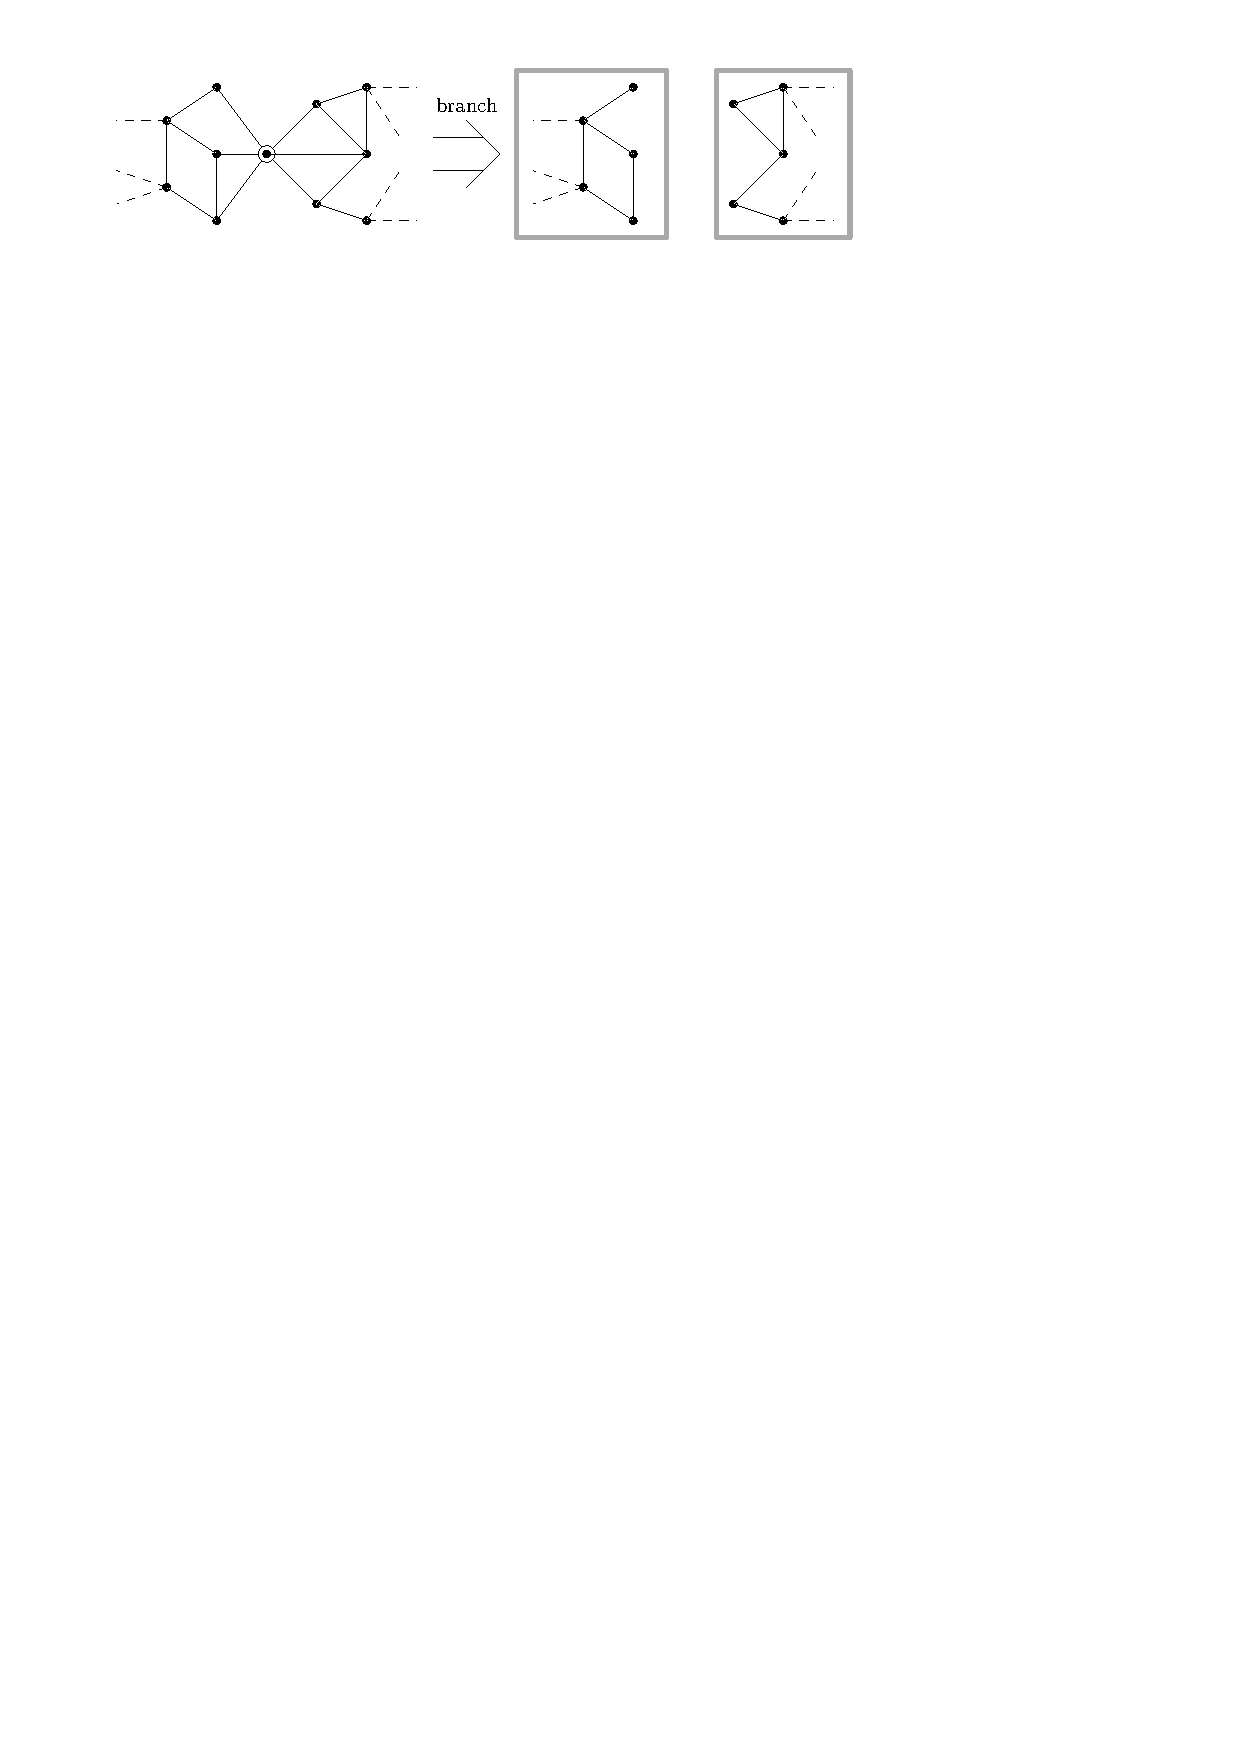
\includegraphics[scale=1]{figures/articulation_points}
  \caption{Branching on an articulation point (circled vertex) the
    graph decomposes into two connected components (gray boxes) that can be
    solved independently. The graphic show the branch on which the vertex is
    excluded from the independent set.}
  \label{fig:articulation_points}
\end{figure}

Even tough this strategy yields only a small (linear) overhead, finding articulation points can be rare depending on the type of graph.
This results in the default branching strategy being selected rather
frequently.
Furthermore, our preliminary experiments indicated that articulation points are rarely found at higher depth.
Thus, we limit the maximum depth at which we search for articulation points.

\subsection{Edge Cuts}
To alleviate the restrictive nature of finding articulation points, we now propose a more flexible branching strategy based on \emph{(minimal) edge cuts}.
In general, we still aim to find small vertex separators, \ie a set of vertices whose removal disconnects the graph.
We do so by making use of minimum edge cuts.

A \emph{cut} $(S,T)$ is a partitioning of $V$ into two sets $S$ and $T=V\setminus S$.
Furthermore, a cut is called minimum if its \emph{cut set} $C = \{\{u,v\} \in E \mid u \in S, v \in T\}$ has minimal cardinality.
However, in practice, finding minimum cuts often yields trivial cuts with either $S$ or $T$ only consisting of a single vertex with minimum degree. 
Thus, we are interested in finding \emph{$s$-$t$-cuts}, \ie cuts where $S$ and $T$ contain specific vertices $s,t \in V$.
Finding these cuts can be done efficiently in practice, \eg using a preflow push algorithm~\cite{goldberg1988new}.
However, selecting the vertices $s$ and $t$ to ensure reasonably balanced cuts can be tricky.
Natural choices include random vertices, as well as vertices that are far apart in terms of their shortest path distance.
However, our preliminary experiments indicate that selecting random vertices of maximum degree
 for $s$ and $t$ seems to produce the best results.
Finally, to derive a vertex separator from a cut one can compute an MVC on the bipartite graph induced by the cut set, \eg using the Hopcroft-Karp algorithm~\cite{hopcroft1973n}.
This separator can then be used to select branching vertices.

Overall, our second strategy works similar to the first one: We maintain a set of possible branching vertices that were selected by computing a minimum $s$-$t$-cut and turning it into a vertex separator.
Vertices that were removed by kernelization are discarded from this set and once it is empty, a new cut computation is started.
However, in contrast to the first strategy finding a set of suitable branching vertices is much more likely.
In order to avoid separators that contain too many vertices, and thus would require too many branching steps to disconnect the graph, we only keep those that do not exceed a certain size and balance threshold.
The specific values for these threshold are presented in Section~\ref{sec:algo_conf}.
Finally, if no suitable separator is found, we use the default branching strategy.
Furthermore, in this case we do not try to find a new separator for a fixed number of branching steps as finding one is both unlikely and costly.

\subsection{Nested Dissection}
Both of our previous strategies dynamically maintain a set of possible branching vertices.
Even though this comes at the advantage that most of the computed vertices remain viable candidates for some branching steps, it introduces a noticeable overhead.
To alleviate this, our last strategy uses a static ordering of possible branching vertices that is computed once at the beginning of the algorithm.
For this purpose we make use of a \emph{nested dissection ordering}~\cite{george1973nested}.

A nested dissection ordering of the vertices of a graph $G$ is obtained by recursively computing balanced bipartitions $(A,B)$ and a vertex separator $S$, that separates $A$ and $B$.
The actual ordering is then given by concatenating the orderings of $A$ and $B$ followed by the vertices of $S$.
Thus, if we select branching vertices based on the reverse nested dissection
ordering, we continuously branch on vertices that disconnect the graph into balanced partitions. 
We compute such an ordering once, after finishing the initial kernelization phase.

There are two main optimizations that we use when considering the nested dissection ordering.
First, we noticed that vertices at the end of the ordering seldom lead to a decomposition of the graph. 
This is due to vertices being removed by kernelization which can lead to separators becoming invalid.
Thus, we limit the number of recursive calls during the nested dissection computation.
Furthermore, similar to the edge cut based strategy, we limit the size of
separators considered during branching using a threshold.
Again, this is done to ensure that we do not require too many branching steps to decompose the graph.
The specific value for this size threshold is given in Section~\ref{sec:algo_conf}.
If any separator in the nested dissection exceeds this threshold, we use the default branching strategy.

\section{Reduction Branching}
\label{sec:reduction_branching}
Our second approach to selecting good branching vertices is to choose a vertex
whose removal will enable the application of new reduction rules. During every
reduction step we find a list of candidate vertices to branch on. The following
sections will demonstrate how we identify such branching candidate vertices with little
computational overhead in practice. To be self contained we will also repeat the reduction
rules used here but omit any proofs that can be found in the original
publications. Out of the candidates found we then select a vertex of
maximum degree. If the degree of all candidate vertices lies below a threshold
(defined in Section~\ref{sec:algo_conf}) or no candidate vertices were found we fall back to branching on a vertex
of maximum degree. The rational here is that a vertex of large degree changes
the structure of the graph more than a vertex of small degree even if that
vertex is guaranteed to enable the application of a reduction rule. Also, our
current strategies only enable the application of the targeted reduction rule in
the branch that excludes the vertex from the independent set. However, in the
case that includes it into the independent set all neighbors are removed from
the graph as well because they already have an adjacent vertex in the solution.

We also did some preliminary experiments with storing the candidate vertices in
a priority queue across branch-reduce steps and updating that list continually.
However, changes where too frequent for this approach to be faster because of
the high amount of priority queue operations compared to the relatively low overhead
caused by the current approach.

\subsection{Almost Twins}

The first reduction we target is the \emph{twin} reduction by Xiao and Nagamochi~\cite{XiaoUnconfined}:

\begin{definition}(Twins~\cite{XiaoUnconfined})
  In a graph $G=(V,E)$ two vertices $u$ and $v$ are called twins, if $N(u) = N(v)$ and $d(u) = d(v) = 3$.
\end{definition}

\begin{theorem} (Twin Reduction~\cite{XiaoUnconfined}) In a graph $G=(V,E)$ let
  vertices $u$ and $v$ be twins. If there is an edge among $N(u)$, then there is
  always an MIS that includes $\{u,v\}$ and therefore
  excludes $N(u)$. Otherwise, let $G'=(V',E')$ be the graph with $V'=(V\setminus
  N[\{u,v\}])\cup\{w\}$ where $w\notin V$ and $E'=(E\cap\binom{V'}{2})\cup
  \{\{w,x\}\;|\;x\in N^2(u)\})\}$ and let $I'$ be an MIS in $G'$. Then, 
  $
  I=\begin{cases}
    I'\cup \{u,v\} & \text{, if }w\notin I'\\
    (I'\setminus \{w\})\cup N(u) & \text{, else} %w\in I'
  \end{cases}
  $
  is an MIS in $G$.
\end{theorem}

We now define \emph{Almost Twins} as follows:
\begin{definition} (Almost Twins)
  In a graph $G=(V,E)$ two non adjacent vertices $u$ and $v$ are called almost twins if $d(u) = 4$, $d(v) = 3$ and $N(v)\subseteq N(u)$ (\ie $N(u) = N(v) \cup \{w\}$). 
\end{definition}

Clearly, after removing $w$, $u$ and $v$ are twins so we can apply the twin
reduction. Finding almost twins can be done while searching for twins: The
original algorithm checks for each vertex $v$ of degree $3$ whether there is a
vertex $u \in N^2(v)$ which $d(u) = 3$ and $N(u) = N(v)$. We augment this
algorithm by simultaneously also searching for $u \in N^2(v)$ with $d(u) = 4$
and $N(v) \subset N(u)$. This induces about the same computational cost for
degree $4$ vertices in $N^2(v)$ as for degree $3$ vertices. While there might be
instances where this causes high overhead, we expect the practical slowdown to
be small. Figure~\ref{fig:twin} illustrates branching for almost twins. 

\begin{figure}[t]
  \centering
  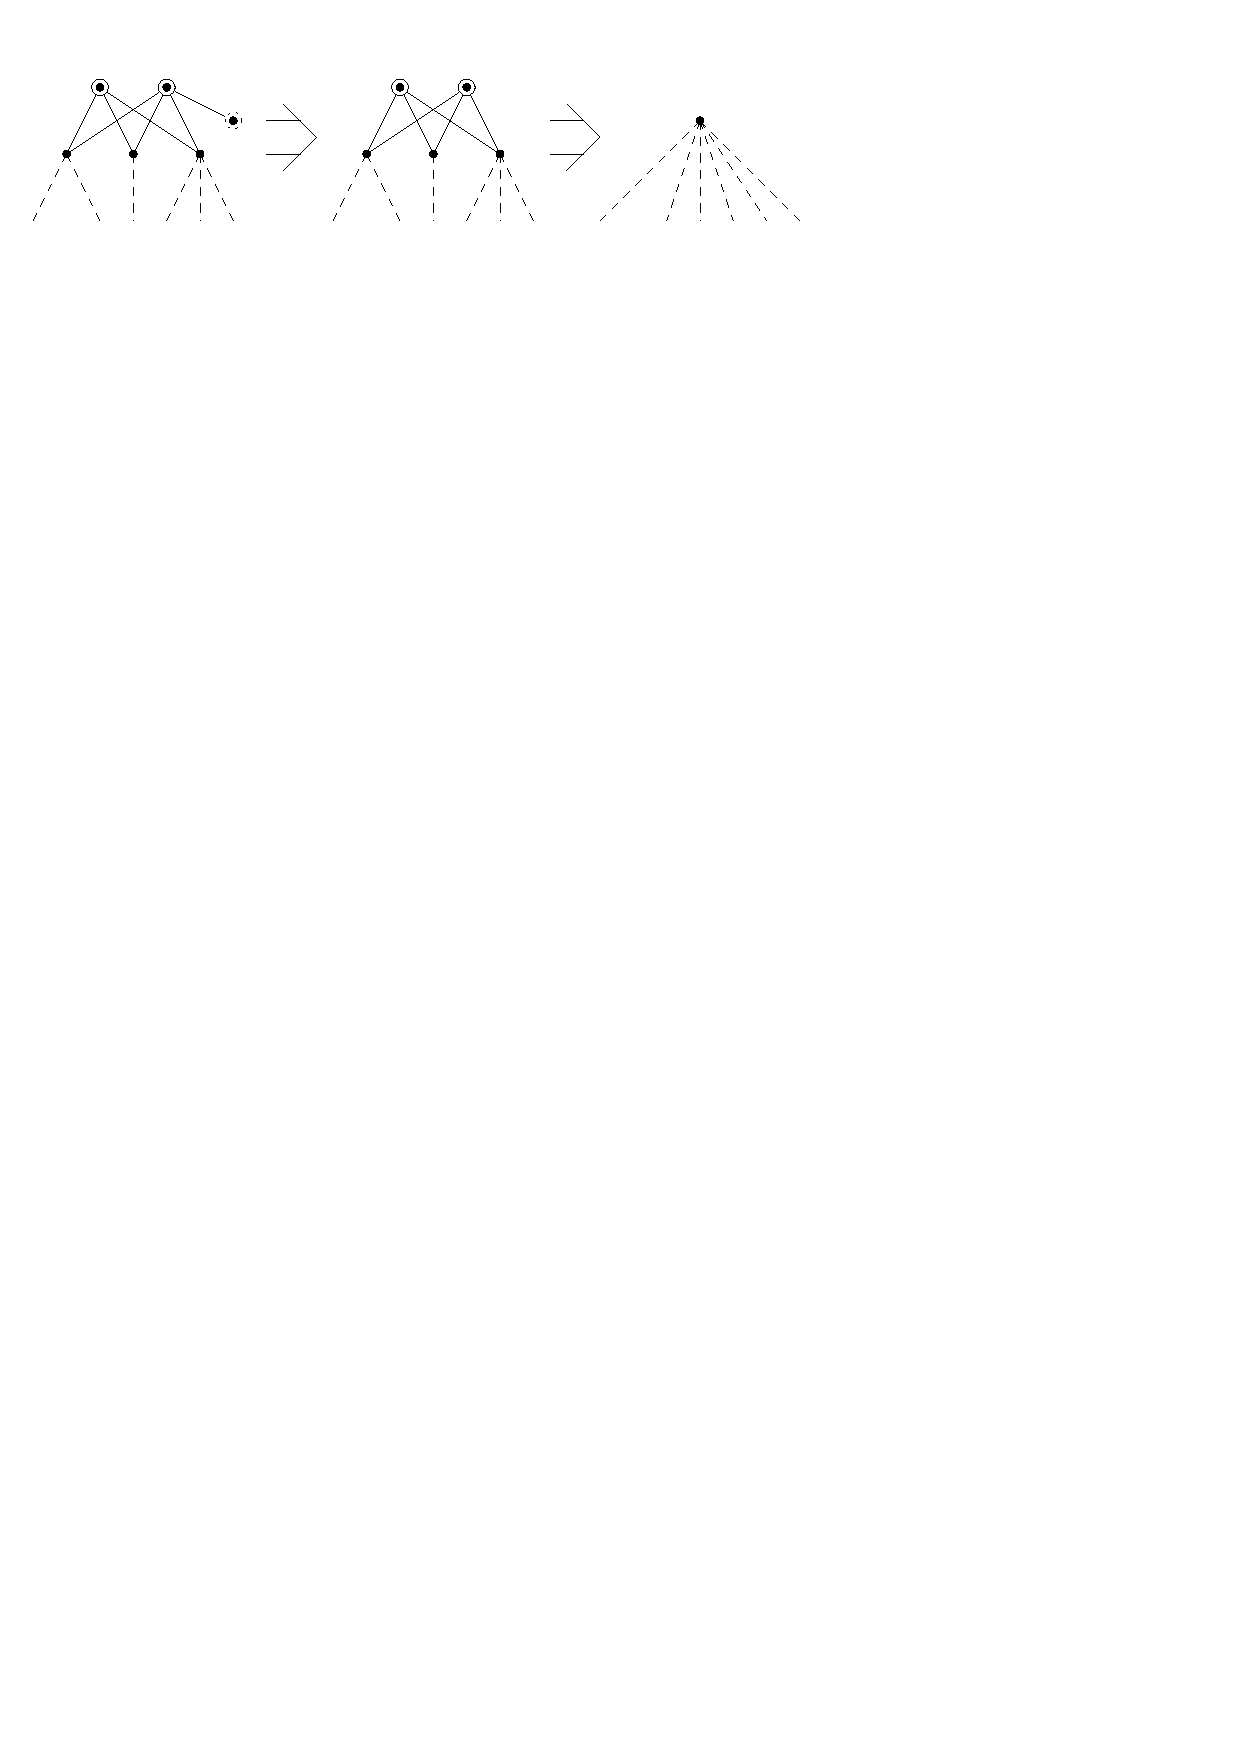
\includegraphics[scale=1]{figures/twin}
  \caption{The two solidly circled vertices are almost twins. After branching on
  the dashed circled vertex they become twins (in the excluding branch) and can
  be reduced.}
  \label{fig:twin}
\end{figure}

\subsection{Almost Funnels}
\label{sec:almost_funnels}

Next we consider the \emph{funnel} reduction which is a special case of the
\emph{alternative} reduction by Xiao and Nagamochi~\cite{XiaoUnconfined}:

\begin{definition} (Alternative Sets~\cite{XiaoUnconfined})
	In a graph $G=(V,E)$ two non empty, disjoint subsets $A,B\subseteq V$ are
    called alternatives, if $|A| = |B|$ and there is an MIS $I$ in $G$ such that $I\cap(A\cup B)$ is either $A$ or $B$.
\end{definition}

\begin{theorem} (Alternative Reduction~\cite{XiaoUnconfined})
	In a graph $G=(V,E)$ let $A$ and $B$ be alternative sets. Let $G'=(V', E')$
    the graph with $V' = V\setminus(A\cup B\cup (N(A)\cap N(B)))$ and $E' =
    \{\{u,v\} \in E \mid u,v \in V'\} \cup \{ \{u,v\}\;|\; u\in
    N(A)\setminus N[B], v\in N(B)\setminus N[A] \}$ and let $I'$ be an MIS in $G'$. Then,
	$
    I=\begin{cases}
      I'\cup A & \text{, if } (N(A)\setminus N[B]) \cap I' = \emptyset% N(B)\setminus N[A]\subseteq I'\\
      \\
      I'\cup B & \text{, else}
	\end{cases}
    $
	is an MIS in $G$.
\end{theorem}

Note that the alternative reduction adds new edges between existing
vertices of the graph which might not be beneficial in every case. To counteract this, the algorithm
by Akiba and Iwata~\cite{AkibaIwata} only uses special cases, one of which is
the funnel reduction:

\begin{definition} (Funnel~\cite{XiaoUnconfined})
	In a graph $G=(V,E)$ two adjacent vertices $u$ and $v$ are called funnels, if $G_{N(v)\setminus\{u\}}$ is a complete graph, i.e, if $N(v)\setminus\{u\}$ is a clique.
\end{definition}
\begin{theorem} (Funnel Reduction~\cite{XiaoUnconfined}) In a graph $G=(V,E)$ let $u$ and $v$ be funnels. Then, $\{u\}$ and $\{v\}$ are alternative sets.	
\end{theorem}

Again, we define a structure that is covered by the funnel reduction after
removal of a single vertex:

\begin{definition}(Almost Funnel)
  In a graph $G=(V,E)$ two adjacent vertices $u$ and $v$ are called almost funnels if $u$ and $v$ are not funnels and there is a vertex $w$ such that $N(v)\setminus\{u,w\}$ induces a clique.
\end{definition}

By removing $w$, $u$ and $v$ become funnels. The original funnel algorithm
checks whether $u$ and $v$ are funnels by iterating over the vertices in $N(v) \setminus \{u\}$
and checking whether they are adjacent to \emph{all} previous vertices. Once a vertex
is found that is not adjacent to all previous vertices, the algorithm concludes
that $u$ and $v$ are not funnels and terminates. We augment this algorithm by
not immediately terminating in this case. Instead, we consider the following two
cases: Either the current vertex $w$ is not adjacent to at least two of the
previous vertices. In this case, we can check whether $N(v) \setminus \{u, w\}$
induces a clique. In the second case, $w$ is adjacent to all but one previous
vertex $w'$. In this case, both $w$ and $w'$ might be candidate branching
vertices. Thus, we check whether $N(v) \setminus \{u, w\}$ or $N(v) \setminus
\{u, w'\}$ induce a clique. This adds up to two additional clique checks (of
slightly smaller size) to the one clique check in the original algorithm.

% \subsection{Almost Dominance}
% \label{sec:almost_dominance}

% The next branching strategy is based on the dominance reduction rule by Fomin et al.~\cite{Fomin}:

% \begin{definition} (Dominance~\cite{Fomin})
%   In a graph $G=(V,E)$ a vertex $u$ is called dominated by a neighbor $v$, if $N[u]\subseteq N[v]$.
% \end{definition}

% \begin{theorem} (Dominance Reduction~\cite{Fomin}) In a graph $G=(V,E)$, if a
%   vertex $u$ is dominated by a neighbor $v$, then, there always exists an MIS that does not include $v$, i.e.~$\alpha(G)=\alpha(G-\{v\})$
% \end{theorem}

% A vertex is almost dominated by one of it has only one surplus neighbor:

% \begin{definition} (Almost Dominance)
%   In a graph $G=(V,E)$ a vertex $u$ is called almost dominated by a neighbor $v$ if $|N(u)\setminus N(v)| = 1$ and $N[v]\not\subseteq N(u)$.
% \end{definition}
%  The last condition ensures that $v$ is not dominated by $u$. The original
%  algorithm checks for each neighbor of $u$ is also a neighbor of $v$. Once it
%  finds a vertex in $N(u)$ that is not in $N(v)$, it terminates because $u$ can not
%  be dominated by $v$. We augment this algorithm by allowing a single vertex $w
%  \in N(u)$ that is not adjacent to $v$ and adding $w$ as a candidate branching
%  vertex if it exists. If $w$ is found early in the algorithm, this might induce
%  some overhead to the algorithm but assuming the position of $w$ in $u$'s
%  adjacency list to be uniformly randomly distributed, the expected number of
%  vertices to check only doubles.

%  Note that the dominance reduction is not directly used in the Algorithm by
%  Akiba and Iwata~\cite{AkibaIwata} because it is fully contained in the unconfined
%  reduction (see Section~\ref{sec:almost_unconfined}). This means that we cannot
%  simply search for almost dominated vertices during the reduction step. Instead,
%  we have to do an additional pass over all vertices.
 
\subsection{Almost Unconfined}
\label{sec:almost_unconfined}

% The \emph{unconfined} reduction by Xiao and Nagamochi~\cite{XiaoNagamochi} is a generalization of the dominance reduction
% (see Section~\ref{sec:almost_dominance}).
The core idea of the \emph{unconfined} reduction by Xiao and
Nagamochi~\cite{XiaoUnconfined} is to detect vertices not required for an MIS
that can therefore can be removed from the graph by algorithmically
contradicting the assumption that every MIS contains the vertex.

\begin{definition} (Removable Vertex~\cite{XiaoUnconfined})
	In a graph $G=(V,E)$ a vertex $v$ is called removable, if 
	$\alpha(G) = \alpha(G-\{v\})$.
\end{definition}

\begin{definition} (Child, Parent~\cite{XiaoUnconfined}) In a graph $G=(V,E)$ with an \textit{independent set} $I$, a vertex $v$ is called a child of $I$, if $|N(v)\cap I| = 1$ and the unique neighbor of $v$ in $I$ is called the parent of $v$.
\end{definition}

\begin{theorem} (\cite{XiaoUnconfined})\label{theorem:unconfined}
	In a graph $G=(V,E)$ let $S$ be an independent set that is not maximal but is contained in every MIS of $G$ and let $v$ be any child of $S$. Then, every MIS includes at least one vertex from $N(v)\setminus N[S]$.
\end{theorem}

Based on Theorem \ref{theorem:unconfined} Algorithm \ref{alg:unconf} detects so called \textit{unconfined} vertices.

\begin{algorithm}[t]
	\caption{Unconfined -- Xiao and Nagamochi
      \cite{XiaoUnconfined}}\label{alg:unconf}
	\SetKwFunction{U}{Unconfined}
	\DontPrintSemicolon
	
	\KwIn{A graph $G$, a vertex $v$}
	\U{G, v}	
	\Begin{
		$S \leftarrow \{v\}$\;
		\While{$S\text{ has child }u\text{ with } |N(u)\setminus N[S]|\leq 1$}{
			\eIf{$|N(u)\setminus N[S]| = 0$}{\Return true\tcp*{contradiction to Theorem \ref{theorem:unconfined}}}{
				$\{w\}\leftarrow N(u)\setminus N[v]$\tcp*{by assumption $w$ also has to}
				$S\leftarrow S\cup\{w\}$\tcp*{be contained in every MIS}
			}
		}
		
		\Return $\text{false}$
		
	}
	
	\KwOut{true if $v$ is unconfined, false otherwise}
	
\end{algorithm}


\begin{theorem}(Unconfined Reduction~\cite{XiaoUnconfined}) In a graph $G=(V,E)$,
  if Algorithm \ref{alg:unconf} returns true for an unconfined vertex $v$, then
  there is always an MIS that does not contain~$v$.
\end{theorem}\todo{Wenn wir Platzprobleme haben, können wir auch nur den Algo
  und dieses Theorem behalten}

Again, we define a vertex to be almost unconfined:

\begin{definition} (Almost Unconfined)
  In a graph $G=(V,E)$ a vertex $v$ is called almost unconfined if $v$ is not unconfined but there is a vertex $w$ such that $v$ is unconfined in $G-\{w\}$.
\end{definition}

Here, we only present an augmentation that detects \emph{some} almost
unconfined vertices. In particular, if at any point during the algorithm there
is only \emph{one} extending child, i.e. a child $u$ of $S$ with $N(u)\setminus
N[S] = \{w\}$, then removal of $w$ makes $v$ unconfined. During
Algorithm~\ref{alg:unconf} we collect all these vertices $w$ and add them to the
set of candidate branching vertices if the algorithm cannot already remove $v$.
This only adds the overhead of temporarily storing the potential candidates and
adding them to the actual candidate list if $v$ is not removed.

% Note that this special case of almost unconfined vertices might not catch all
% cases of almost dominated vertices.

\section{Experimental Evaluation}

In this section we present the results of our experimental evaluation. Tables
and figures here show aggregated results. For
detailed results for all of our algorithms across all instances, see Appendix~\ref{app:detailed_results}.

\subsection{Experimental Environment}
We execute all our experiments on a machine with 4 8-core Intel Xeon E5-4640 CPUs
(2.4~GHz) and 512 GiB DDR3-PC1600 RAM. To speed up our experiments we use two
identical machines and run \textcolor{red}{X}\todo{@Christian: How many} instances at once on the
same machine (using the same machine for all algorithms on a specific instance).
All numbers reported are averages \todo{@Christian or means?} of three runs with
a timeout of \textcolor{red}{X}\todo{@Christian: fill in} hours.

\subsection{Algorithm Configuration}
\label{sec:algo_conf}
We use a C++ adaptation of the implementation by Akiba and
Iwata~\cite{AkibaIwata} in its default configuration\todo{@Christian: Is this
  true?} as a basis for our algorithm. During preliminary experiments we found
suitable values for the parameters of
our techniques. These experiments were run on a subset of our total instance
set. We use the geometric mean over all instances of the speedup over the
default branching strategy as a basis for our decision: The number of branching
steps skipped after an unsuccessful search for articulation points is set
to \textcolor{red}{X}\todo{@Christian: fill in}. For the technique based on
s-t-cuts, we only use cuts that contain at most
\textcolor{red}{X}\todo{@Christian: fill in} vertices and where the smaller side of
the cut contains at least \textcolor{red}{X}\todo{@Christian: fill in} vertices.
If no suitable separator is found, we skip \textcolor{red}{X}\todo{@Christian:
  fill in} branching steps. For computing nested dissections, we use 
InertialFlowCutter\footnote{\url{https://github.com/kit-algo/InertialFlowCutter}}
with the KaHIP\footnote{\url{https://kahip.github.io/}}
backend.\todo{@Christian: Add parameters for this.} For branching we use
\textcolor{red}{X}\todo{@Christian: fill in} levels of nested dissections and
only use the nested dissection if separators contain at most
\textcolor{red}{X}\todo{@Christian: fill in} vertices. For the reduction based
branching rules, we fall back to the default branching strategy if all
candidates have a degree of less than \textcolor{red}{X}\todo{@Christian: fill in}.

\subsection{Instances}
We use instances from several sources: A sample of the instances used for the
PACE 2019 Challenge on Minimum Vertex Cover~\cite{dzulfikar_et_al:LIPIcs:2019:11486}. Maximum Clique instances from the second
DIMACS Implementation Challenge~\cite{johnson1993cliques} and sparse instances from
the Stanford Network Analysis Project (SNAP)~\cite{snapnets}\todo{@Christian:
  Ich kann hier nicht alle Graphen aus der Liste finden. Außerdem: Muss man für
  die Instanzen noch andere Sachen zitieren?}.\todo{road networks mit Quelle?} Detailed instance information can
be found in Appendix~\ref{app:instances}.\todo{@Christian: Add table of
  instances with num. vertices and edges.}

\subsection{Decomposition Branching}
\label{sec:experiments_decomp}

\todo{@Sebastian: Da decomposition based so schlecht funktioniert, sollten wir
  vielleicht im Hauptteil und hier die beiden Ansätze tauschen?}
Figure~\ref{fig:all_decomp_time} shows a perfomance plot of the running time of
our decomposition based branching strategies: For each instance, the best
algorithm is determined. The plot shows for each algorithm $1$ minus the time of the best algorithm
divided by the time the respective algorithm took. So a value of $0$ means that
the algorithm was the fastest algorithm on that instance and a value of
$\numprint{0.5}$ means that the algorithm took twice as long as the fastest
algorithm. Timeouts are shown as a value $> 1$. For each algorithm, instances
are then sorted by their value. Note that this means that the points on a
vertical line do not correspond to the same instance.

The plot shows that for most instances, the default strategy of branching on a
vertex of maximum degree outperforms our decomposition based approaches.
However, there is one instance\todo{Update after full results are in} (web-stanford) that causes a timeout with the
default strategy but can be solved in $48$\todo{Update after full results are in} (articulation points) to $176$\todo{Update after full results are in} (nested
dissections) seconds using a decomposition based approach. Accounting a time of
\textcolor{red}{timeouttime}\todo{insert timeout} for the default strategy on
this instance, this results in a geometric mean speedup of about two for all
decomposition based techniques on the SNAP instances (see Table~\ref{tab:summary_decomp}).\todo{@christian:
  Interpretiere ich diese Zahl richtig?} Overall, most running
times are only slightly slower than the default strategy. This is mainly because
the number of branches required to solve the instances does not change in most
cases (see Figure~\ref{fig:all_decomp_branch}) and most of the running time
difference is caused by the overhead from
searching for branching vertices. Table~\ref{tab:summary_decomp} \dots\todo{write
  something about the table}

\begin{table}[t]
  \caption{Speedup of our decomposition based techniques over the default
    strategy (max. degree). ``all'' are geometric means of the speedup over all
  instances of that type (timeouts are assigned a running time of
  \textcolor{red}{timeouttime} hours), ``solved'' are geometric means of the
  speedup over all instances that have been solved by all techniques.}
\label{tab:summary_decomp}

  \centering
  \begin{tabular}{|l|rr|rr|rr|rr|}
    \hline
    Instance type $\rightarrow$ & \multicolumn{2}{c|}{PACE} & \multicolumn{2}{c|}{DIMACS} & \multicolumn{2}{c|}{SNAP} & \multicolumn{2}{c|}{All Instances}                                                                                                          \\
    technique $\downarrow$      & \multicolumn{1}{c}{all}   & \multicolumn{1}{c|}{solved} & \multicolumn{1}{c}{all}   & \multicolumn{1}{c|}{solved} & \multicolumn{1}{c}{all} & \multicolumn{1}{c|}{solved} & \multicolumn{1}{c}{all} & \multicolumn{1}{c|}{solved} \\
    \hline
    articulation points         & \textcolor{red}{TODO}     & \textcolor{red}{TODO}       & \textcolor{red}{TODO}     & \textcolor{red}{TODO}       & \textcolor{red}{TODO}   & \textcolor{red}{TODO}       & \textcolor{red}{TODO}   & \textcolor{red}{TODO}       \\
    st-cuts                     & \textcolor{red}{TODO}     & \textcolor{red}{TODO}       & \textcolor{red}{TODO}     & \textcolor{red}{TODO}       & \textcolor{red}{TODO}   & \textcolor{red}{TODO}       & \textcolor{red}{TODO}   & \textcolor{red}{TODO}       \\
    nested dissections          & \textcolor{red}{TODO}     & \textcolor{red}{TODO}       & \textcolor{red}{TODO}     & \textcolor{red}{TODO}       & \textcolor{red}{TODO}   & \textcolor{red}{TODO}       & \textcolor{red}{TODO}   & \textcolor{red}{TODO}       \\
    \hline
    \end{tabular}
\end{table}

\begin{figure}[t]
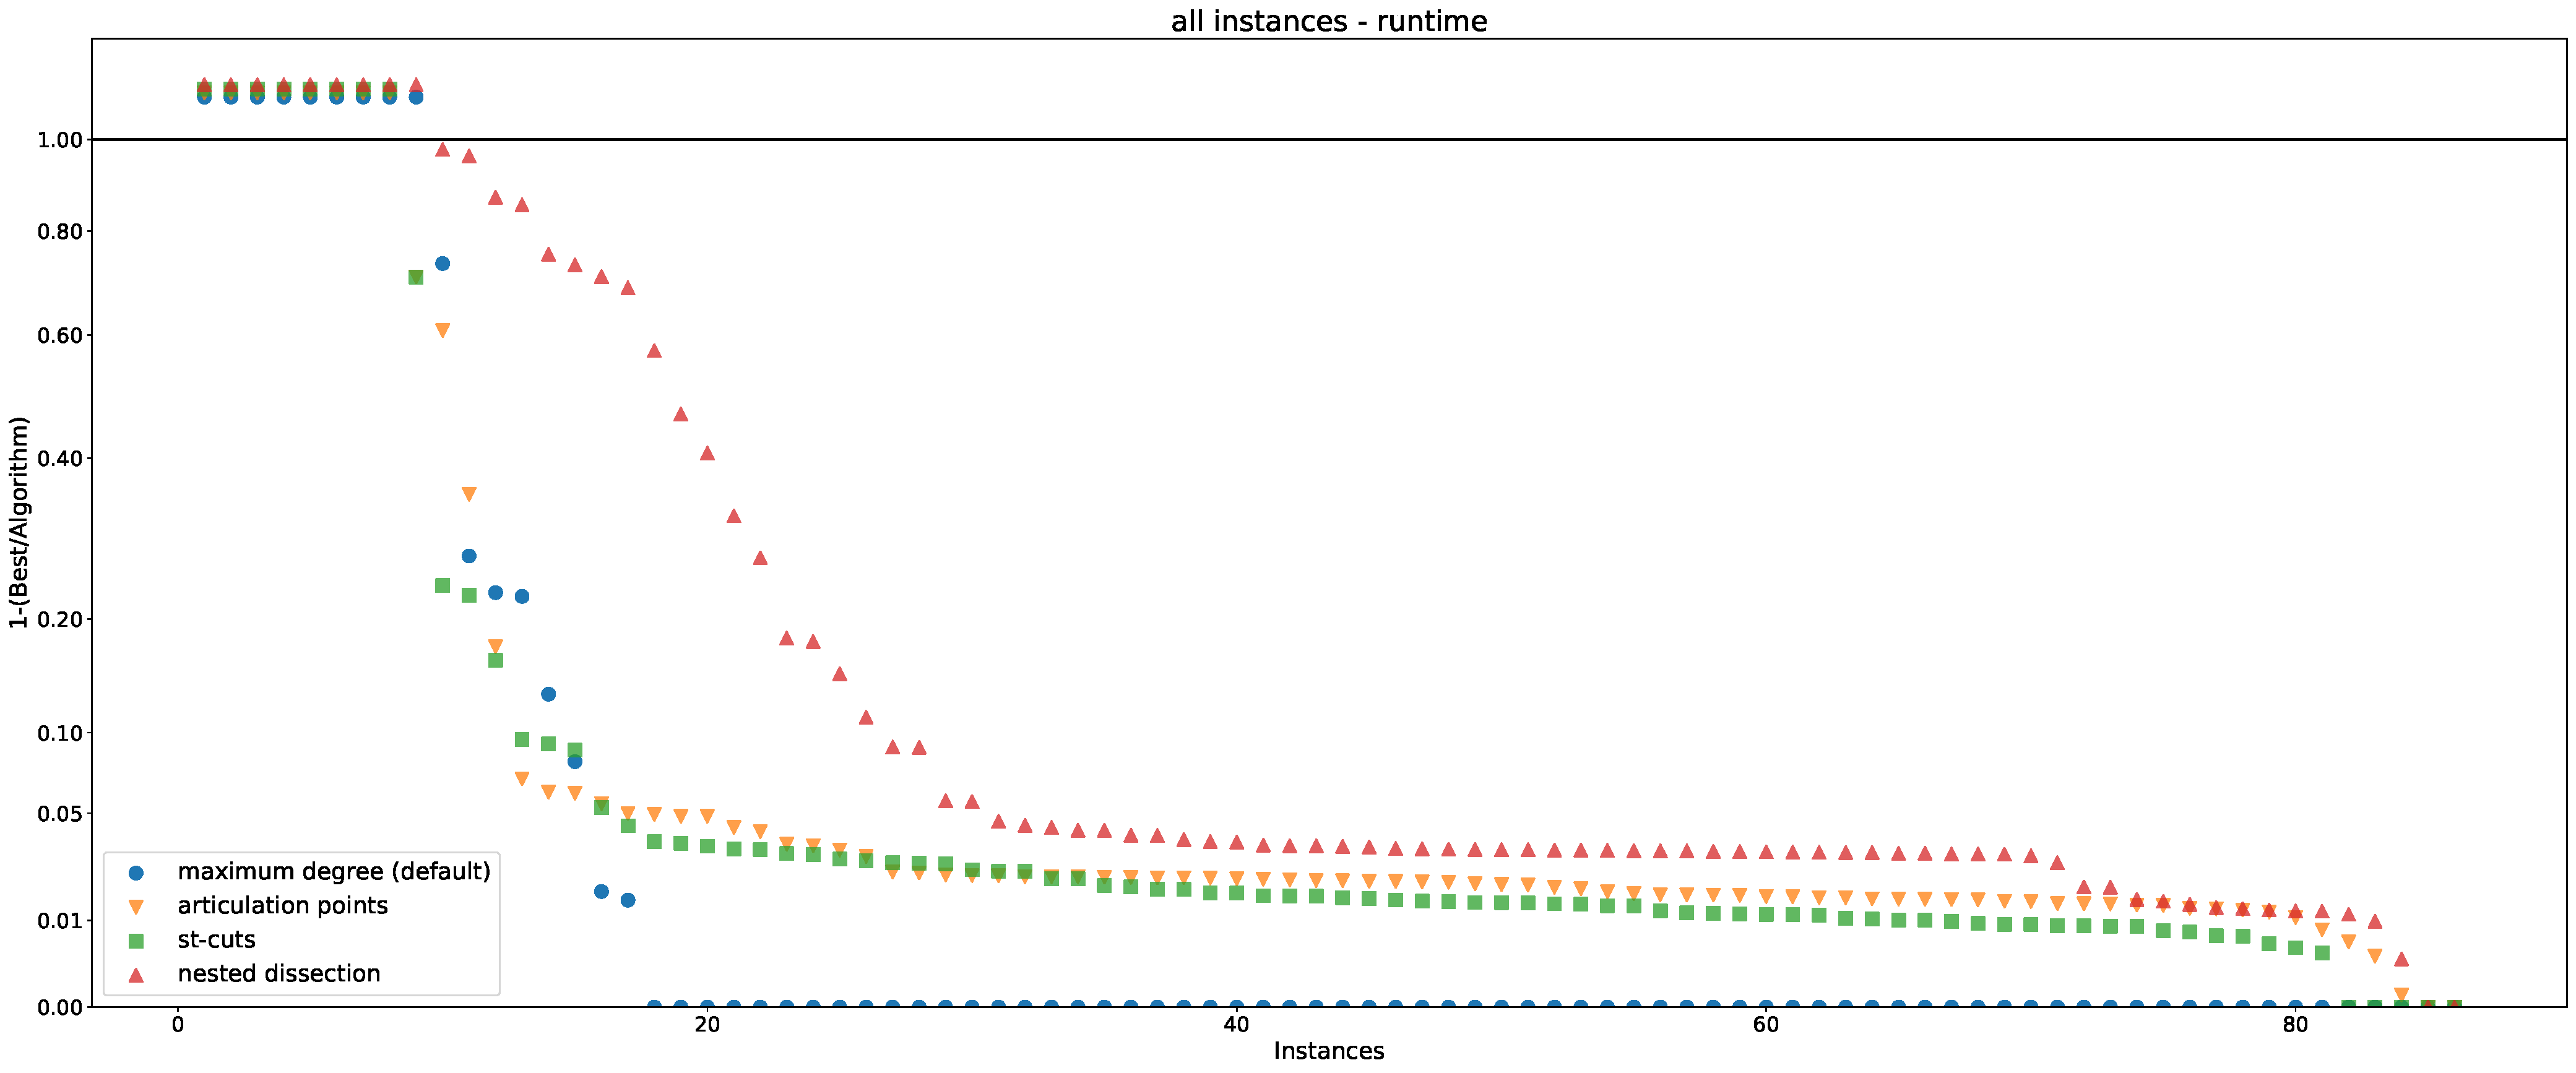
\includegraphics[width=\textwidth]{plots/all_decomposition_based_time}
\caption{Performance plot comparing running times of decomposition based branching strategies.}
\label{fig:all_decomp_time}
\end{figure}

\begin{figure}[t]
  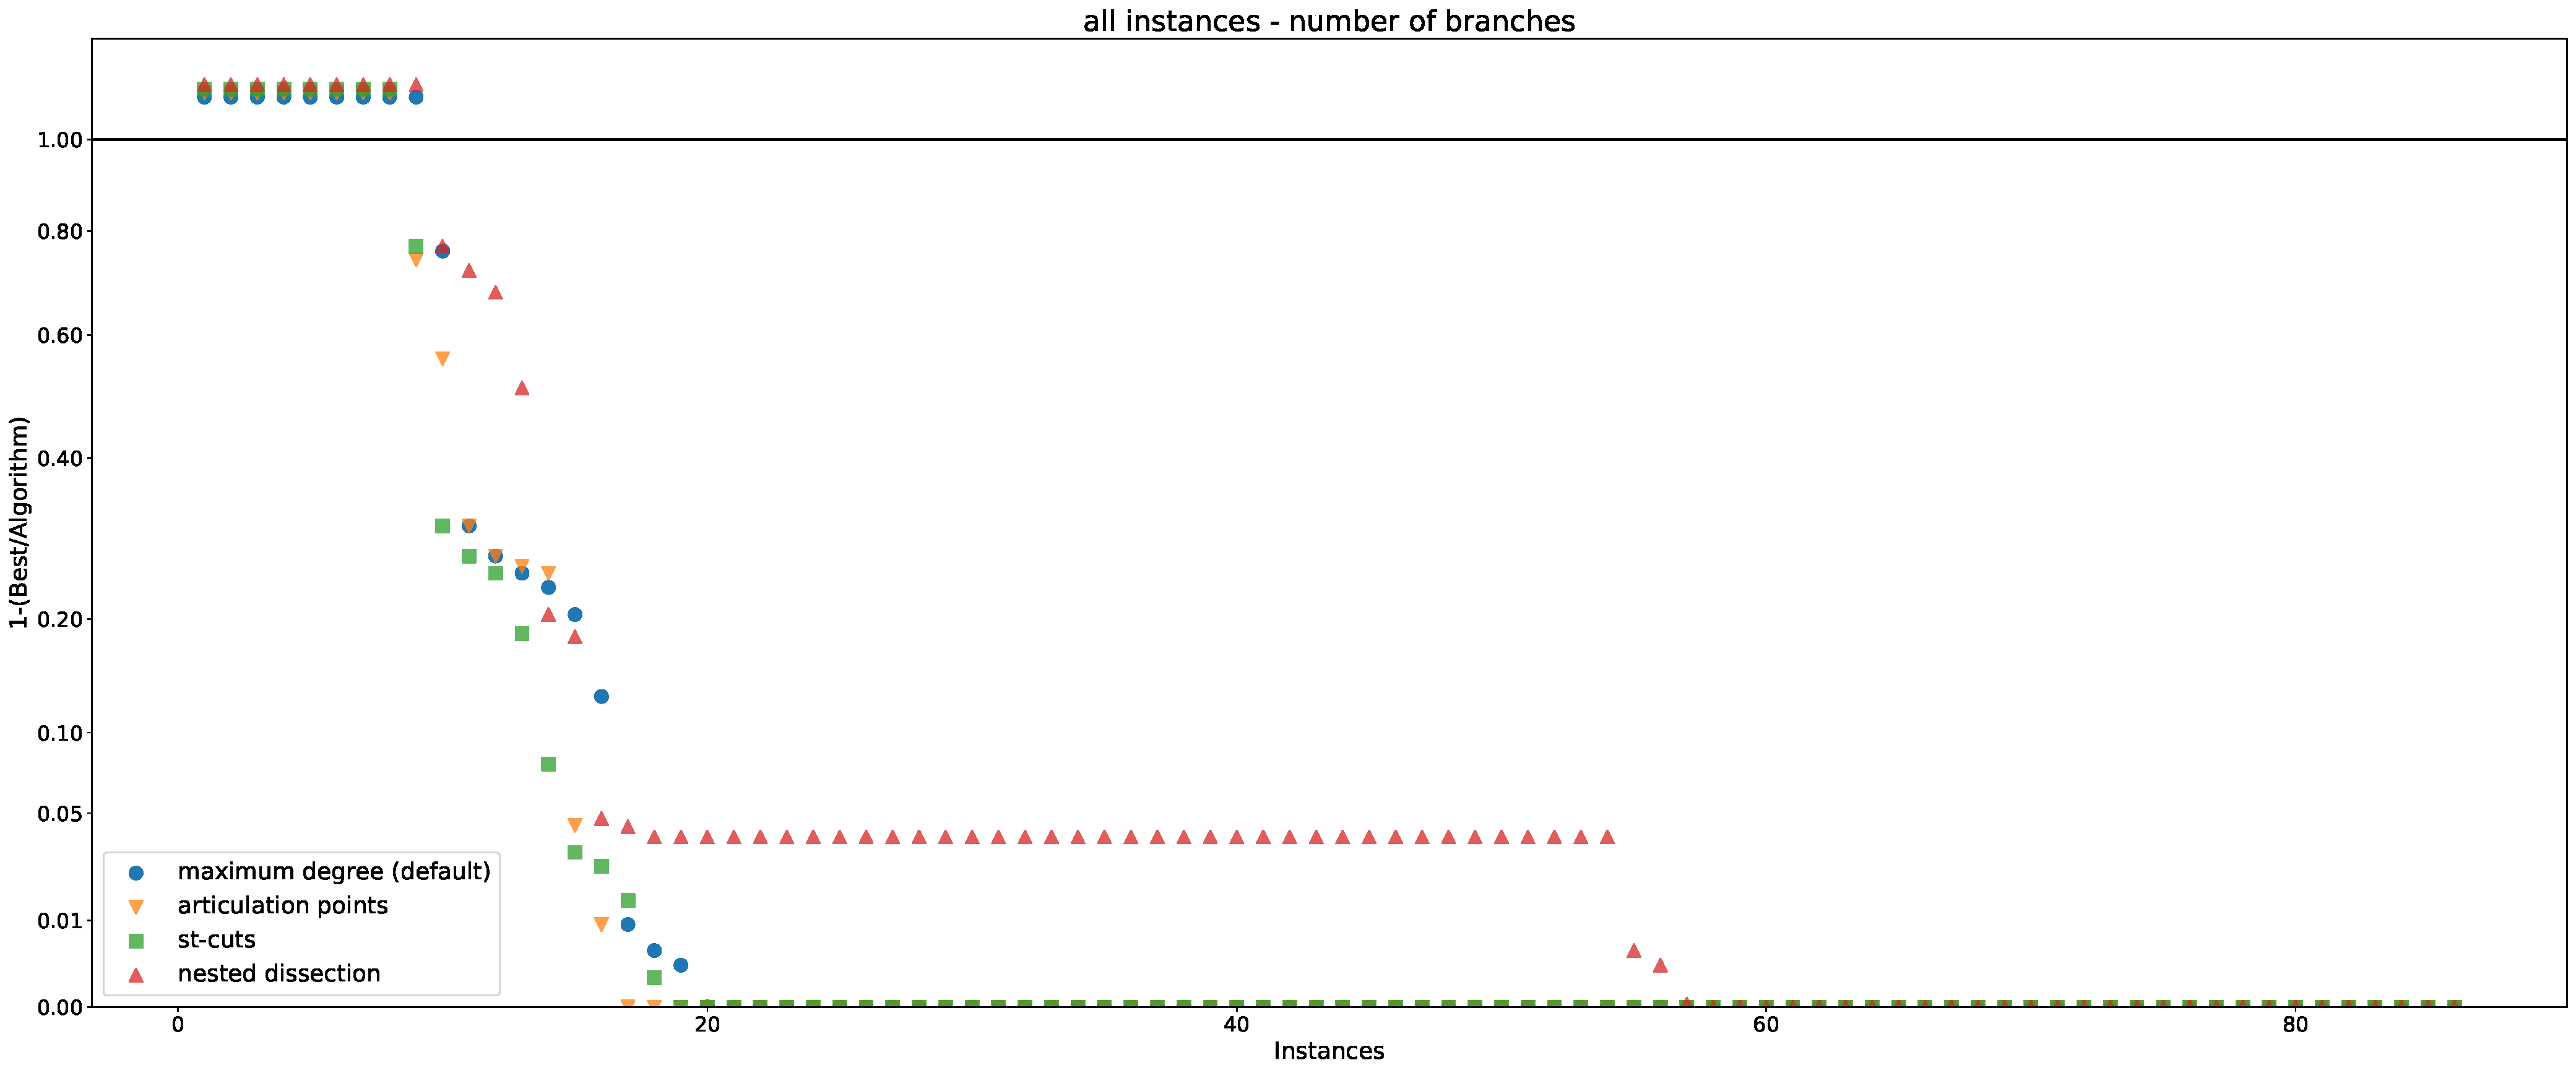
\includegraphics[width=\textwidth]{plots/all_decomposition_based_branch}
  \caption{Performance plot comparing branches of decomposition based branching strategies.}
  \label{fig:all_decomp_branch}
\end{figure}


% \FloatBarrier
\subsection{Reduction Branching}
Figure~\ref{fig:all_reduction_time} shows the performance plot (see
Section~\ref{sec:experiments_decomp}) for our reduction
based branching strategies. Here we see that targeting the funnel reduction
results in the fastest time for the most number of instances. In fact, the
funnel based technique is the fastest for all but 9 of the PACE instances. The
default strategy is only fastest for 4 of these instances. However, all
reduction based strategies fail to solve instance 40 of the PACE dataset which
the default strategy solves in about 7 hours\todo{update with final number}.
Interestingly, when targeting the funnel reduction, PACE instance 36 times out
but can be solved in 10 to 83 seconds\todo{update numbers} with all other
strategies. We also show results for a strategy that targets all reduction rules
described in Section~\ref{sec:reduction_branching}. Even though this approach
leads to the lowest number of branches for most instances (see Figure~\ref{fig:all_reduction_branch}), the time required to
identify candidate vertices for all reduction rules causes too big of an
overhead to be competitive. Optimizing the algorithms to identify candidate
vertices could lead to making this combined strategy
dominant. Table~\ref{tab:summary_reduction} \dots\todo{write
  something about the table}

\begin{table}[t]
  \caption{Speedup of our reduction based techniques over the default
    strategy (max. degree). ``all'' are geometric means of the speedup over all
  instances of that type (timeouts are assigned a running time of
  \textcolor{red}{timeouttime} hours), ``solved'' are geometric means of the
  speedup over all instances that have been solved by all techniques.}
\label{tab:summary_reduction}

  \centering
  \begin{tabular}{|l|rr|rr|rr|rr|}
    \hline
    Instance type $\rightarrow$ & \multicolumn{2}{c|}{PACE} & \multicolumn{2}{c|}{DIMACS} & \multicolumn{2}{c|}{SNAP} & \multicolumn{2}{c|}{All Instances}                                                                                                          \\
    reduction rule $\downarrow$ & \multicolumn{1}{c}{all}   & \multicolumn{1}{c|}{solved} & \multicolumn{1}{c}{all}   & \multicolumn{1}{c|}{solved} & \multicolumn{1}{c}{all} & \multicolumn{1}{c|}{solved} & \multicolumn{1}{c}{all} & \multicolumn{1}{c|}{solved} \\
    \hline
    Twin                        & \textcolor{red}{TODO}     & \textcolor{red}{TODO}       & \textcolor{red}{TODO}     & \textcolor{red}{TODO}       & \textcolor{red}{TODO}   & \textcolor{red}{TODO}       & \textcolor{red}{TODO}   & \textcolor{red}{TODO}       \\
    Funnel                      & \textcolor{red}{TODO}     & \textcolor{red}{TODO}       & \textcolor{red}{TODO}     & \textcolor{red}{TODO}       & \textcolor{red}{TODO}   & \textcolor{red}{TODO}       & \textcolor{red}{TODO}   & \textcolor{red}{TODO}       \\
    Unconfined                  & \textcolor{red}{TODO}     & \textcolor{red}{TODO}       & \textcolor{red}{TODO}     & \textcolor{red}{TODO}       & \textcolor{red}{TODO}   & \textcolor{red}{TODO}       & \textcolor{red}{TODO}   & \textcolor{red}{TODO}       \\
    Combined                    & \textcolor{red}{TODO}     & \textcolor{red}{TODO}       & \textcolor{red}{TODO}     & \textcolor{red}{TODO}       & \textcolor{red}{TODO}   & \textcolor{red}{TODO}       & \textcolor{red}{TODO}   & \textcolor{red}{TODO}       \\
    \hline
    \end{tabular}
\end{table}

\begin{figure}[t]
  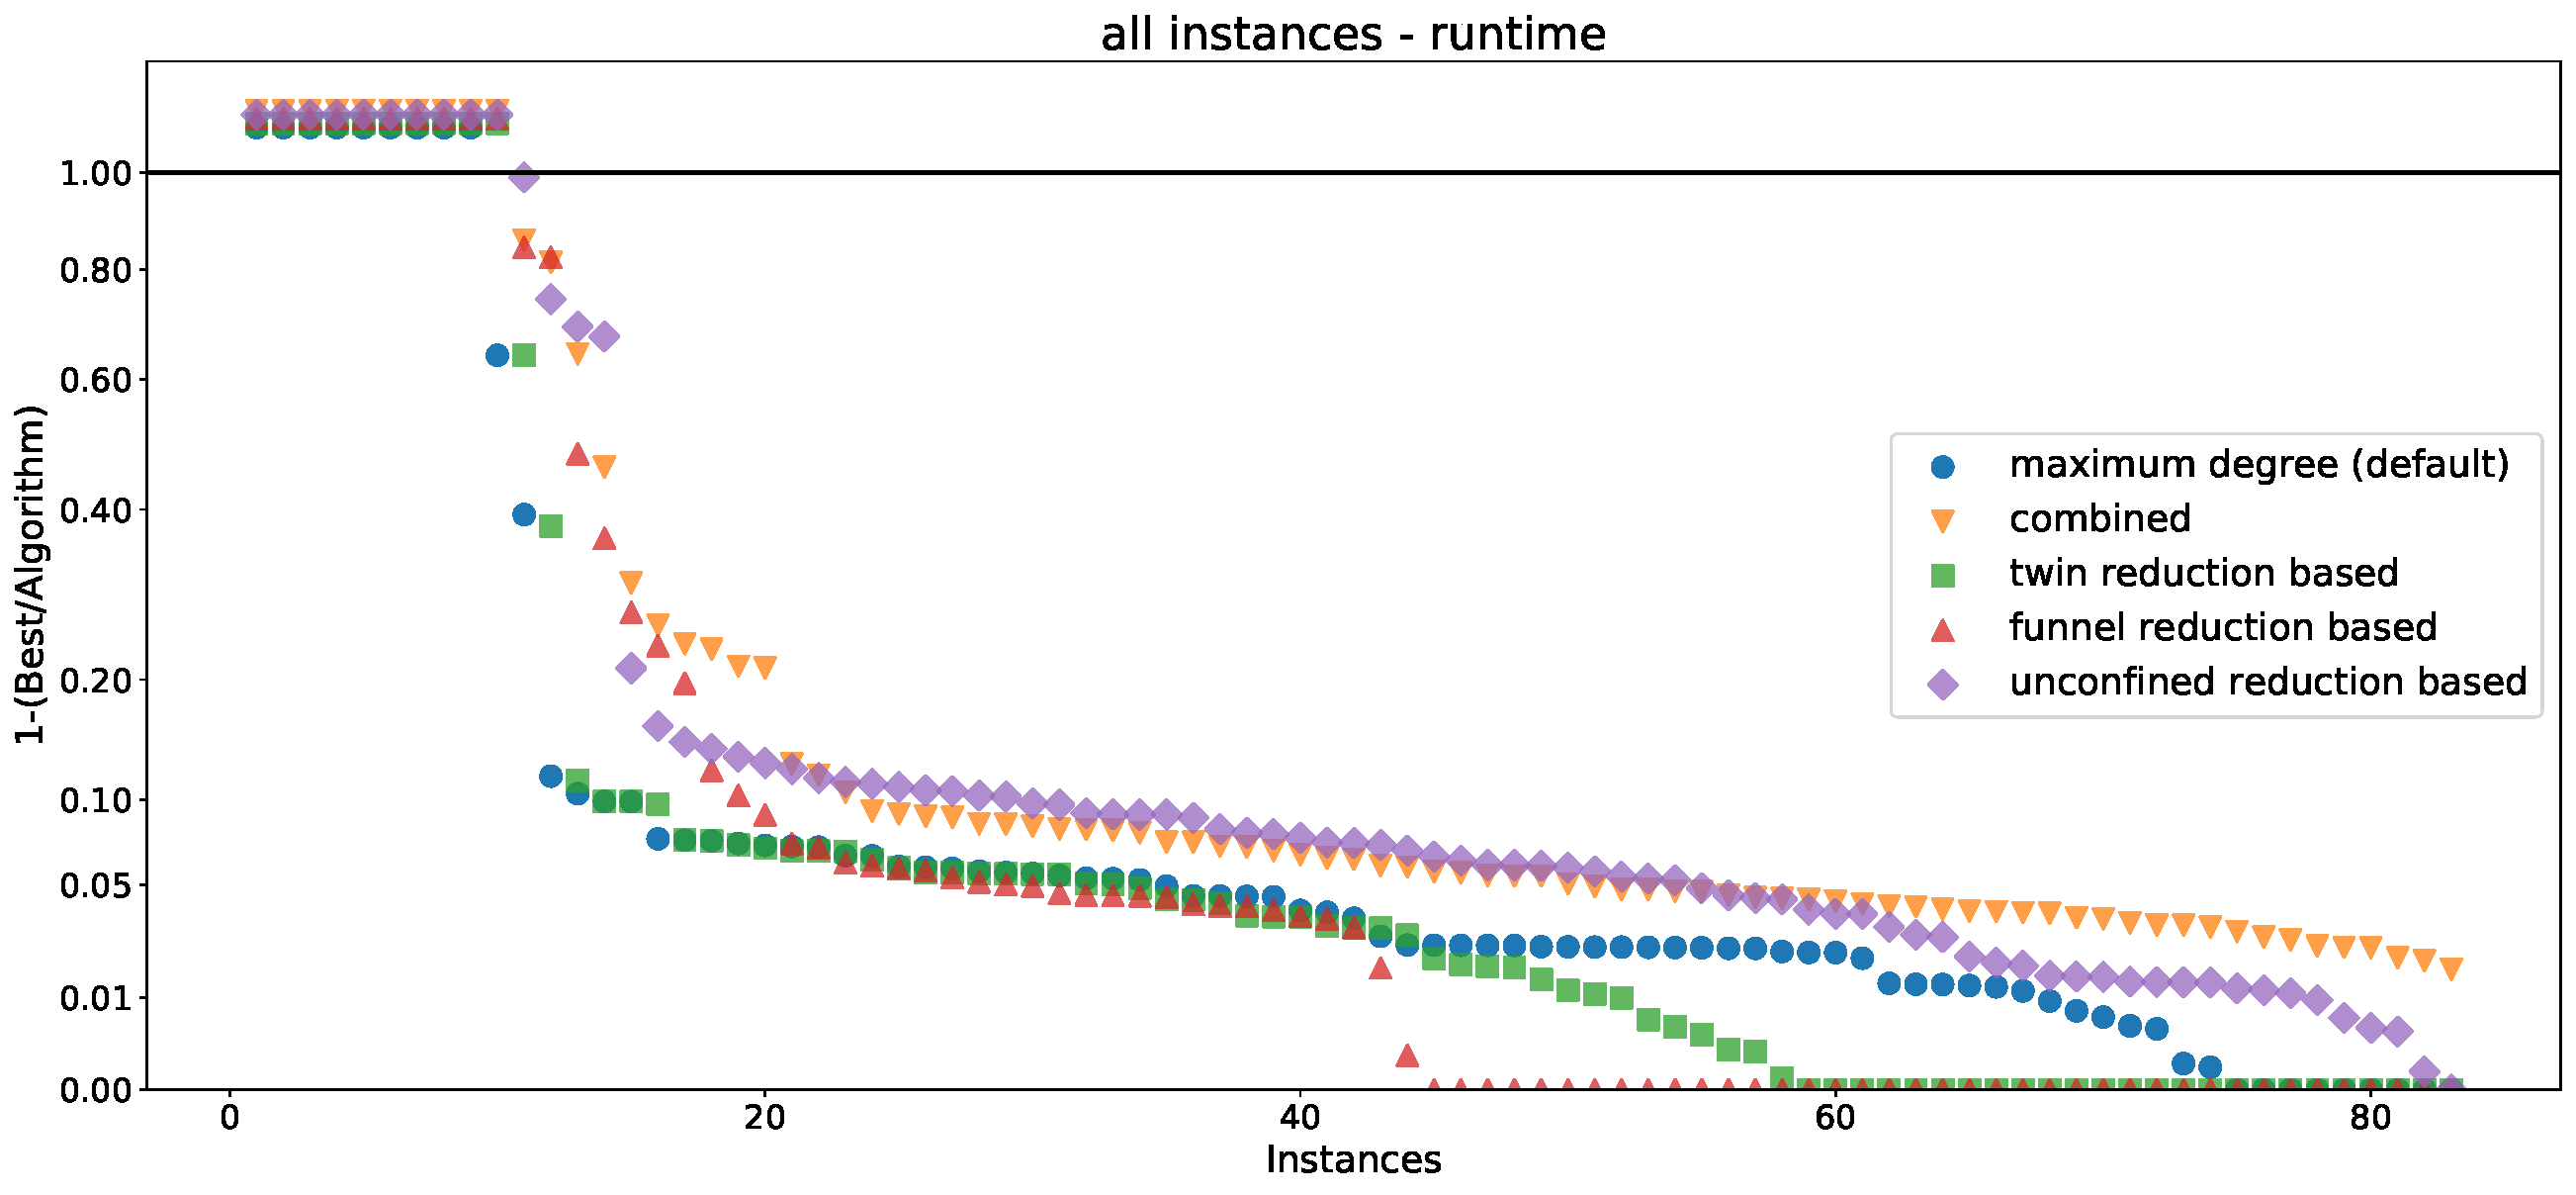
\includegraphics[width=\textwidth]{plots/all_reduction_based_time}
  \caption{Performance plot comparing running time of reduction based branching strategies.}
  \label{fig:all_reduction_time}
\end{figure}

\begin{figure}[t]
  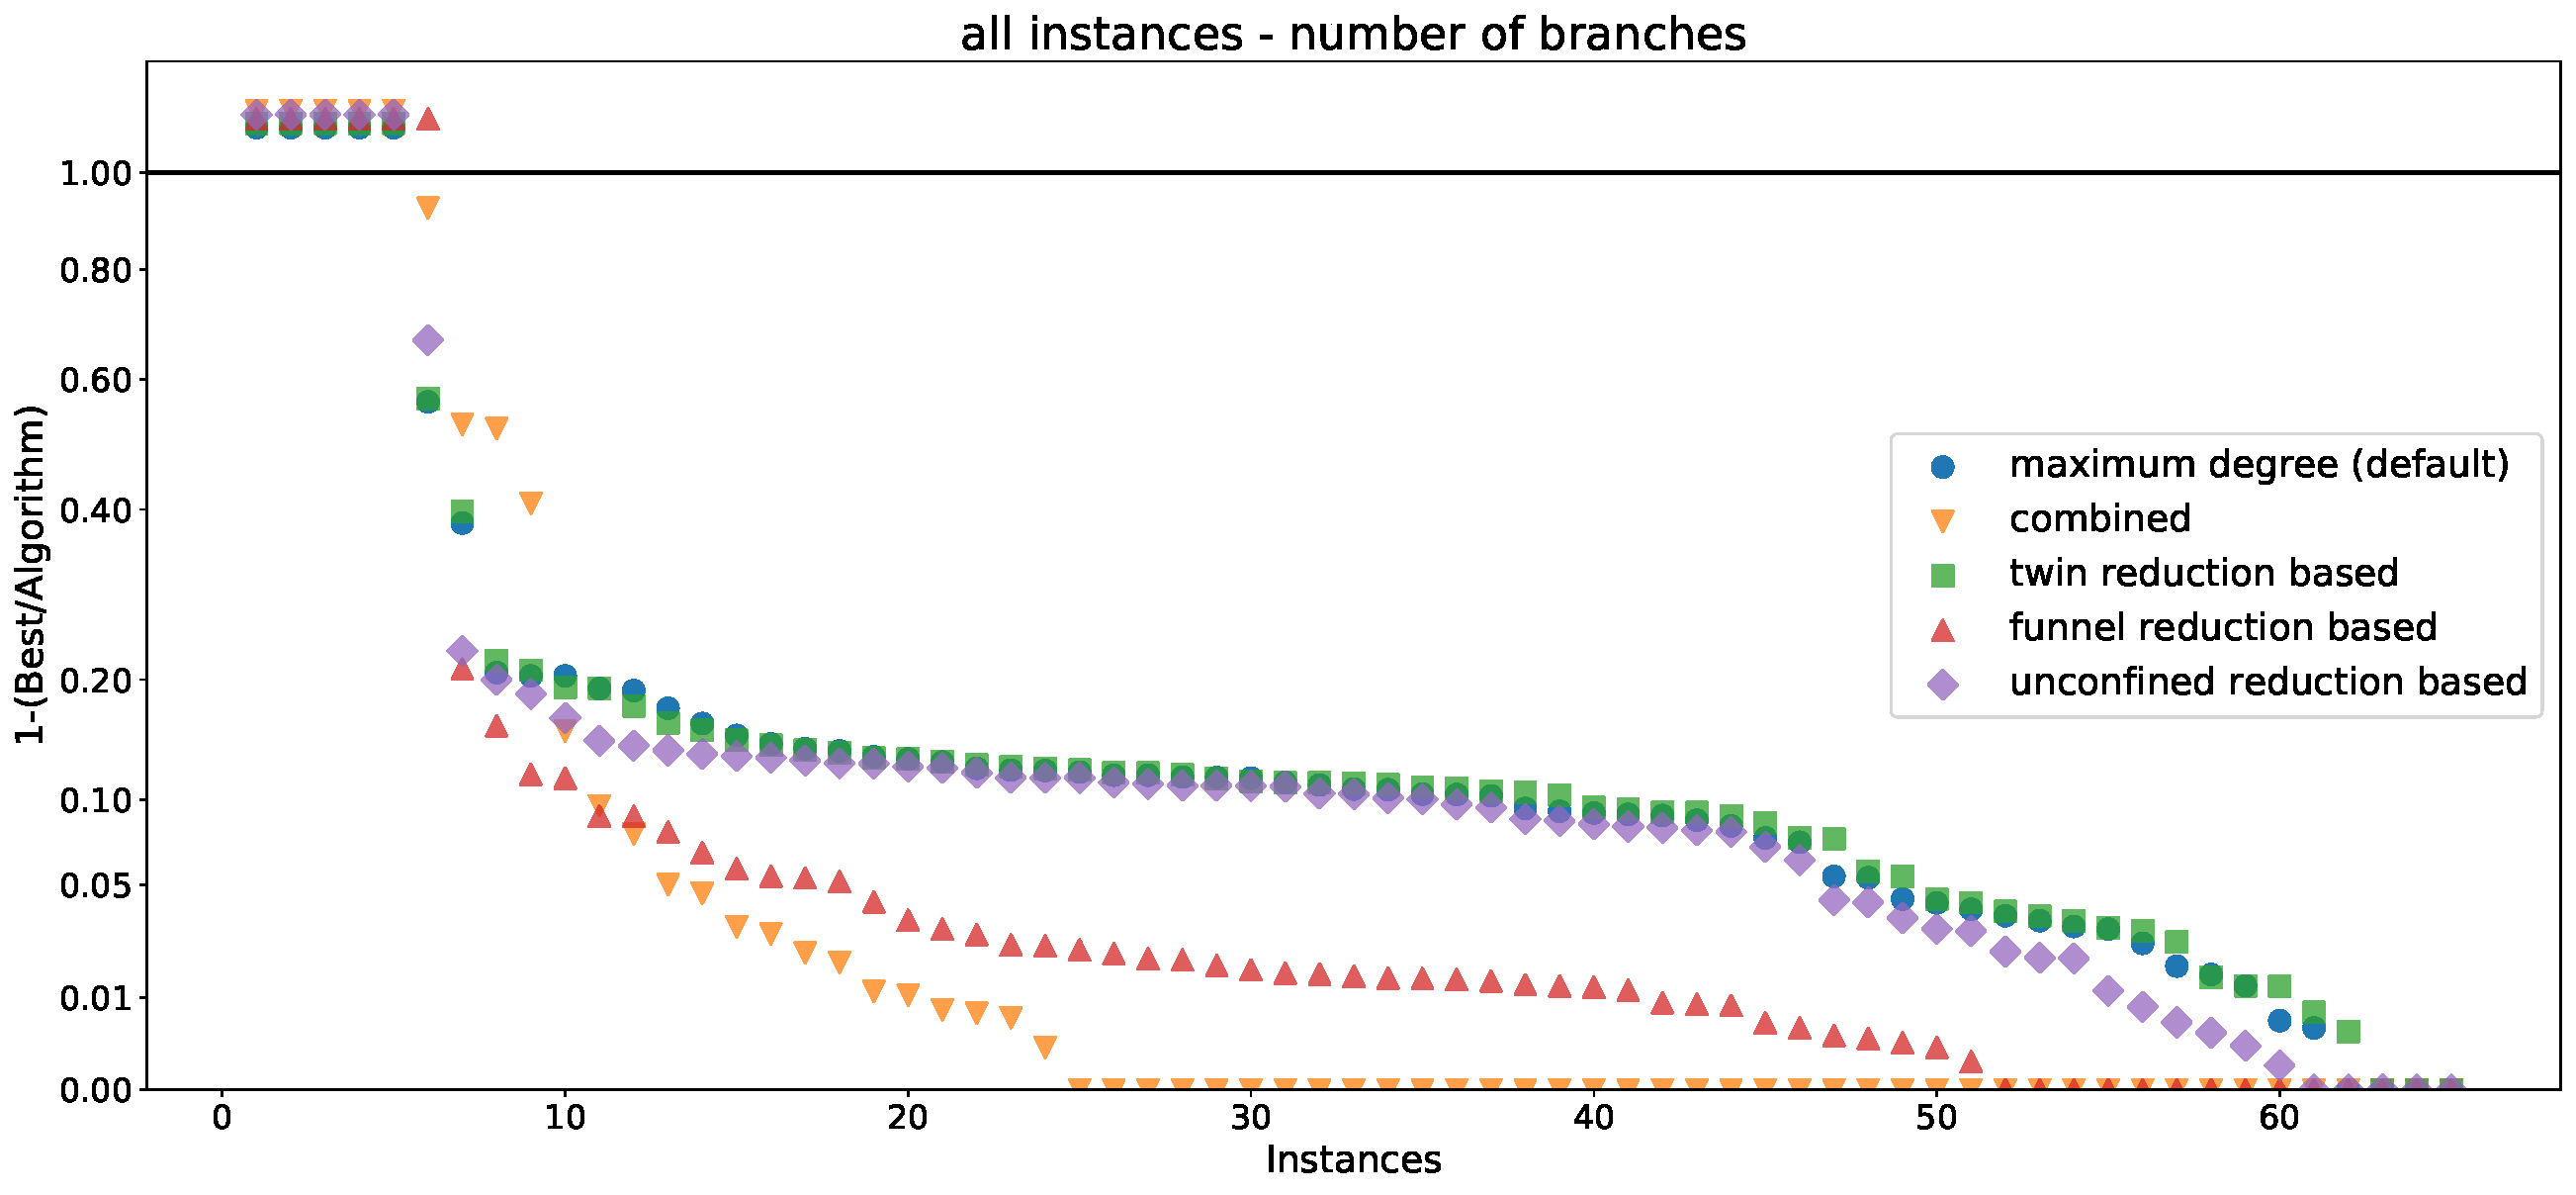
\includegraphics[width=\textwidth]{plots/all_reduction_based_branch}
  \caption{Performance plot comparing branches of reduction based branching strategies.}
  \label{fig:all_reduction_branch}
\end{figure}


\section{Conclusion and Future Work}

%%
%% Bibliography
%%

\FloatBarrier
%% Please use bibtex, 
\todo{TODO: Before submitting check for all references whether they are actually used in the text}
\bibliography{references}

\newpage

\appendix

\section{Detailed Instance Information}
\label{app:instances}
\todo{@Christian: Add table}

\newpage
\section{Detailed Experimental Results}
\label{app:detailed_results}
\todo{@Christian: Kriegen wir die Tabelle auf die gleiche Seite, wie die überschrift?}
\begin{table}
	\small
	\setlength\tabcolsep{2pt} 
	\begin{center}
		\begin{tabular}{|l|r|rr|rr|rr|}\hline
			Graph & max. deg. & Artik. &  & st-cuts &  & ND &  \\
			\hline
			PACE & t (s) & t (s) & s & t (s) & s & t (s) & s \\
			\hline
			36 & \textbf{\numprint{10.67}} & \numprint{10.81} & \numprint{1.01} & \numprint{10.72} & \numprint{1.00} & \numprint{13.02} & \numprint{1.22} \\
			37 & \textbf{\numprint{60.62}} & \numprint{61.64} & \numprint{1.02} & \numprint{61.31} & \numprint{1.01} & \numprint{63.09} & \numprint{1.04} \\
			38 & \numprint{70.79} & \numprint{64.41} & \numprint{0.91} & \textbf{\numprint{18.80}} & \textbf{\numprint{0.27}} & \numprint{76.09} & \numprint{1.07} \\
			39 & \textbf{\numprint{559.85}} & \numprint{567.92} & \numprint{1.01} & \numprint{563.61} & \numprint{1.01} & \numprint{578.62} & \numprint{1.03} \\
			40 & \textbf{\numprint{27278.42}} & \numprint{27624.74} & \numprint{1.01} & \numprint{27385.12} & \numprint{1.00} & \numprint{28154.28} & \numprint{1.03} \\
			41 & \textbf{\numprint{282.83}} & \numprint{288.96} & \numprint{1.02} & \numprint{286.14} & \numprint{1.01} & \numprint{292.02} & \numprint{1.03} \\
			42 & \textbf{\numprint{215.43}} & \numprint{220.05} & \numprint{1.02} & \numprint{218.00} & \numprint{1.01} & \numprint{222.76} & \numprint{1.03} \\
			43 & \textbf{\numprint{1015.97}} & \numprint{1036.92} & \numprint{1.02} & \numprint{1030.05} & \numprint{1.01} & \numprint{1048.52} & \numprint{1.03} \\
			44 & \textbf{\numprint{545.48}} & \numprint{557.95} & \numprint{1.02} & \numprint{554.30} & \numprint{1.02} & \numprint{563.41} & \numprint{1.03} \\
			45 & \textbf{\numprint{147.99}} & \numprint{151.41} & \numprint{1.02} & \numprint{150.04} & \numprint{1.01} & \numprint{153.29} & \numprint{1.04} \\
			46 & \textbf{\numprint{634.70}} & \numprint{643.85} & \numprint{1.01} & \numprint{640.22} & \numprint{1.01} & \numprint{655.75} & \numprint{1.03} \\
			47 & \textbf{\numprint{342.88}} & \numprint{348.28} & \numprint{1.02} & \numprint{346.03} & \numprint{1.01} & \numprint{354.46} & \numprint{1.03} \\
			48 & \textbf{\numprint{147.66}} & \numprint{149.99} & \numprint{1.02} & \numprint{148.81} & \numprint{1.01} & \numprint{152.95} & \numprint{1.04} \\
			49 & \textbf{\numprint{104.01}} & \numprint{105.73} & \numprint{1.02} & \numprint{105.03} & \numprint{1.01} & \numprint{107.91} & \numprint{1.04} \\
			50 & \textbf{\numprint{285.75}} & \numprint{290.25} & \numprint{1.02} & \numprint{288.28} & \numprint{1.01} & \numprint{295.53} & \numprint{1.03} \\
			51 & \textbf{\numprint{330.87}} & \numprint{338.28} & \numprint{1.02} & \numprint{335.72} & \numprint{1.01} & \numprint{341.83} & \numprint{1.03} \\
			52 & \textbf{\numprint{129.84}} & \numprint{132.89} & \numprint{1.02} & \numprint{131.71} & \numprint{1.01} & \numprint{134.53} & \numprint{1.04} \\
			53 & \textbf{\numprint{351.55}} & \numprint{359.29} & \numprint{1.02} & \numprint{356.87} & \numprint{1.02} & \numprint{363.08} & \numprint{1.03} \\
			54 & \textbf{\numprint{189.21}} & \numprint{193.49} & \numprint{1.02} & \numprint{192.39} & \numprint{1.02} & \numprint{195.56} & \numprint{1.03} \\
			55 & \textbf{\numprint{40.08}} & \numprint{41.02} & \numprint{1.02} & \numprint{40.70} & \numprint{1.02} & \numprint{41.87} & \numprint{1.04} \\
			56 & \textbf{\numprint{563.85}} & \numprint{572.37} & \numprint{1.02} & \numprint{568.09} & \numprint{1.01} & \numprint{582.32} & \numprint{1.03} \\
			57 & \textbf{\numprint{391.92}} & \numprint{398.06} & \numprint{1.02} & \numprint{395.36} & \numprint{1.01} & \numprint{404.95} & \numprint{1.03} \\
			58 & \textbf{\numprint{280.57}} & \numprint{285.11} & \numprint{1.02} & \numprint{283.15} & \numprint{1.01} & \numprint{290.23} & \numprint{1.03} \\
			59 & \textbf{\numprint{78.11}} & \numprint{79.44} & \numprint{1.02} & \numprint{78.90} & \numprint{1.01} & \numprint{81.13} & \numprint{1.04} \\
			60 & \textbf{\numprint{466.65}} & \numprint{474.19} & \numprint{1.02} & \numprint{471.02} & \numprint{1.01} & \numprint{482.30} & \numprint{1.03} \\
			61 & \textbf{\numprint{128.58}} & \numprint{131.53} & \numprint{1.02} & \numprint{130.71} & \numprint{1.02} & \numprint{133.14} & \numprint{1.04} \\
			62 & \textbf{\numprint{386.85}} & \numprint{395.27} & \numprint{1.02} & \numprint{392.36} & \numprint{1.01} & \numprint{399.27} & \numprint{1.03} \\
			63 & \textbf{\numprint{400.81}} & \numprint{409.70} & \numprint{1.02} & \numprint{406.70} & \numprint{1.01} & \numprint{413.82} & \numprint{1.03} \\
			64 & \textbf{\numprint{173.83}} & \numprint{177.79} & \numprint{1.02} & \numprint{176.40} & \numprint{1.01} & \numprint{179.85} & \numprint{1.03} \\
			65 & \textbf{\numprint{212.66}} & \numprint{217.21} & \numprint{1.02} & \numprint{215.30} & \numprint{1.01} & \numprint{219.83} & \numprint{1.03} \\
			66 & \textbf{\numprint{47.47}} & \numprint{48.29} & \numprint{1.02} & \numprint{47.97} & \numprint{1.01} & \numprint{49.64} & \numprint{1.05} \\
			67 & \textbf{\numprint{708.92}} & \numprint{718.20} & \numprint{1.01} & \numprint{713.74} & \numprint{1.01} & \numprint{732.34} & \numprint{1.03} \\
			68 & \textbf{\numprint{50.67}} & \numprint{51.40} & \numprint{1.01} & \numprint{50.94} & \numprint{1.01} & \numprint{52.87} & \numprint{1.04} \\
			69 & \textbf{\numprint{252.39}} & \numprint{255.92} & \numprint{1.01} & \numprint{254.63} & \numprint{1.01} & \numprint{261.30} & \numprint{1.04} \\
			70 & \textbf{\numprint{68.24}} & \numprint{69.29} & \numprint{1.02} & \numprint{68.93} & \numprint{1.01} & \numprint{71.01} & \numprint{1.04} \\
			71 & \textbf{\numprint{208.63}} & \numprint{213.05} & \numprint{1.02} & \numprint{210.80} & \numprint{1.01} & \numprint{215.74} & \numprint{1.03} \\
			72 & \textbf{\numprint{269.53}} & \numprint{275.26} & \numprint{1.02} & \numprint{272.72} & \numprint{1.01} & \numprint{278.66} & \numprint{1.03} \\
			73 & \textbf{\numprint{251.79}} & \numprint{257.52} & \numprint{1.02} & \numprint{255.57} & \numprint{1.01} & \numprint{260.38} & \numprint{1.03} \\
			74 & \textbf{\numprint{41.27}} & \numprint{42.22} & \numprint{1.02} & \numprint{41.96} & \numprint{1.02} & \numprint{43.06} & \numprint{1.04} \\
			75 & - & - & - & - & - & - & - \\
			\hline
			$t_{avg}$ (all) & \textbf{\numprint{1843.18}} & \numprint{1856.49} &  & \numprint{1847.48} &  & \numprint{1874.01} & \\
			$s_{geom}$ (all) & \numprint{1.00} & \numprint{1.02} &  & \textbf{\numprint{0.98}} &  & \numprint{1.04} &  \\
			$t_{avg}$ (fin.) & \textbf{\numprint{967.37}} & \numprint{981.02} &  & \numprint{971.77} &  & \numprint{998.98} &  \\
			$s_{geom}$ (fin.) & \numprint{1.00} & \numprint{1.02} &  & \textbf{\numprint{0.98}} & & \numprint{1.04} &  \\
			\hline
		\end{tabular}
	\end{center}
	\caption{Decomposition based strategies - PACE}
	\label{table:another_table}
\end{table}
\begin{table}
	\begin{center}
		\begin{tabular}{|l|r|rr|rr|rr|}\hline
			Graph & max. deg. & Artik. &  & st-cuts &  & ND &  \\
			\hline
			DIMACS & t (s) & t (s) & s & t (s) & s & t (s) & s \\
			\hline
			C125 & \textbf{\numprint{5.49}} & \numprint{5.62} & \numprint{1.02} & \numprint{5.68} & \numprint{1.04} & \numprint{6.03} & \numprint{1.10} \\
			C250 & - & - & - & - & - & - & - \\
			MANN\_a27 & \textbf{\numprint{3.05}} & \numprint{3.11} & \numprint{1.02} & \numprint{3.17} & \numprint{1.04} & \numprint{3.58} & \numprint{1.17} \\
			MANN\_a45 & \textbf{\numprint{473.07}} & \numprint{480.19} & \numprint{1.02} & \numprint{488.14} & \numprint{1.03} & \numprint{479.79} & \numprint{1.01} \\
			MANN\_a9 & \textbf{\numprint{0.00}} & \numprint{0.00} & \numprint{1.07} & \numprint{0.00} & \numprint{1.10} & \numprint{0.07} & \numprint{43.79} \\
			brock200\_1 & \textbf{\numprint{790.54}} & \numprint{805.51} & \numprint{1.02} & \numprint{803.13} & \numprint{1.02} & \numprint{802.48} & \numprint{1.02} \\
			brock200\_2 & \textbf{\numprint{27.00}} & \numprint{28.39} & \numprint{1.05} & \numprint{27.92} & \numprint{1.03} & \numprint{32.82} & \numprint{1.22} \\
			brock200\_3 & \textbf{\numprint{134.07}} & \numprint{136.48} & \numprint{1.02} & \numprint{136.43} & \numprint{1.02} & \numprint{140.52} & \numprint{1.05} \\
			brock200\_4 & \textbf{\numprint{167.00}} & \numprint{169.84} & \numprint{1.02} & \numprint{170.28} & \numprint{1.02} & \numprint{173.32} & \numprint{1.04} \\
			c-fat200-1 & \textbf{\numprint{0.75}} & \numprint{0.79} & \numprint{1.05} & \numprint{0.90} & \numprint{1.19} & \numprint{5.19} & \numprint{6.88} \\
			c-fat200-5 & \textbf{\numprint{0.09}} & \numprint{0.09} & \numprint{1.05} & \numprint{0.12} & \numprint{1.31} & \numprint{2.31} & \numprint{26.26} \\
			gen200\_p0 & \textbf{\numprint{822.73}} & \numprint{852.78} & \numprint{1.04} & \numprint{846.15} & \numprint{1.03} & \numprint{833.19} & \numprint{1.01} \\
			hamming6-4 & \textbf{\numprint{0.14}} & \numprint{0.14} & \numprint{1.04} & \numprint{0.15} & \numprint{1.11} & \numprint{0.48} & \numprint{3.43} \\
			hamming8-4 & \textbf{\numprint{129.50}} & \numprint{135.30} & \numprint{1.04} & \numprint{133.14} & \numprint{1.03} & \numprint{137.20} & \numprint{1.06} \\
			johnson16-2-4 & \textbf{\numprint{236.42}} & \numprint{242.22} & \numprint{1.02} & \numprint{240.87} & \numprint{1.02} & \numprint{239.57} & \numprint{1.01} \\
			johnson8-2-4 & \textbf{\numprint{0.01}} & \numprint{0.01} & \numprint{1.06} & \numprint{0.01} & \numprint{1.10} & \numprint{0.07} & \numprint{7.76} \\
			johnson8-4-4 & \textbf{\numprint{0.37}} & \numprint{0.39} & \numprint{1.06} & \numprint{0.38} & \numprint{1.03} & \numprint{1.38} & \numprint{3.72} \\
			keller4 & \textbf{\numprint{15.94}} & \numprint{16.75} & \numprint{1.05} & \numprint{16.40} & \numprint{1.03} & \numprint{17.94} & \numprint{1.13} \\
			p\_hat1000-1 & \textbf{\numprint{5498.84}} & \numprint{5517.79} & \numprint{1.00} & \numprint{5640.30} & \numprint{1.03} & \numprint{5605.71} & \numprint{1.02} \\
			p\_hat1000-2 & - & - & - & - & - & - & - \\
			p\_hat1500-1 & - & - & - & - & - & - & - \\
			p\_hat300-1 & \textbf{\numprint{25.36}} & \numprint{25.94} & \numprint{1.02} & \numprint{26.52} & \numprint{1.05} & \numprint{47.59} & \numprint{1.88} \\
			p\_hat300-2 & \textbf{\numprint{34.20}} & \numprint{34.77} & \numprint{1.02} & \numprint{35.31} & \numprint{1.03} & \numprint{50.36} & \numprint{1.47} \\
			p\_hat300-3 & \textbf{\numprint{1124.48}} & \numprint{1138.15} & \numprint{1.01} & \numprint{1147.00} & \numprint{1.02} & \numprint{1146.45} & \numprint{1.02} \\
			p\_hat500-1 & \textbf{\numprint{251.75}} & \numprint{255.29} & \numprint{1.01} & \numprint{261.24} & \numprint{1.04} & \numprint{276.61} & \numprint{1.10} \\
			p\_hat500-2 & \textbf{\numprint{593.16}} & \numprint{613.28} & \numprint{1.03} & \numprint{608.09} & \numprint{1.03} & \numprint{611.76} & \numprint{1.03} \\
			p\_hat500-3 & - & - & - & - & - & - & - \\
			p\_hat700-1 & \textbf{\numprint{1035.72}} & \numprint{1044.02} & \numprint{1.01} & \numprint{1066.74} & \numprint{1.03} & \numprint{1065.20} & \numprint{1.03} \\
			p\_hat700-2 & \textbf{\numprint{5675.42}} & \numprint{5707.71} & \numprint{1.01} & \numprint{5775.82} & \numprint{1.02} & \numprint{5745.93} & \numprint{1.01} \\
			san1000 & \textbf{\numprint{6738.26}} & \numprint{6947.83} & \numprint{1.03} & \numprint{6864.69} & \numprint{1.02} & \numprint{6843.53} & \numprint{1.02} \\
			san200\_0 & \textbf{\numprint{1290.60}} & \numprint{1316.67} & \numprint{1.02} & \numprint{1319.54} & \numprint{1.02} & \numprint{1307.43} & \numprint{1.01} \\
			san400\_0 & \textbf{\numprint{12826.58}} & \numprint{12964.68} & \numprint{1.01} & \numprint{13112.91} & \numprint{1.02} & \numprint{12975.06} & \numprint{1.01} \\
			sanr200\_0 & \textbf{\numprint{2144.20}} & \numprint{2187.94} & \numprint{1.02} & \numprint{2198.09} & \numprint{1.03} & \numprint{2170.73} & \numprint{1.01} \\
			\hline
			$t_{avg}$ (all) & \textbf{\numprint{5577.11}} & \numprint{5594.90} & & \numprint{5603.91} & & \numprint{5597.65} &  \\
			$s_{geom}$ (all) & \textbf{\numprint{1.00}} & \numprint{1.03} & & \numprint{1.05} &  & \numprint{1.71} & \\
			$t_{avg}$ (fin.) & \textbf{\numprint{1380.85}} & \numprint{1401.09} & & \numprint{1411.35} &  & \numprint{1404.22} & \\
			$s_{geom}$ (fin.) & \textbf{\numprint{1.00}} & \numprint{1.03} & & \numprint{1.05} & & \numprint{1.71} &  \\
			\hline
		\end{tabular}
	\end{center}
	\caption{Decomposition based strategies - DIMACS}
	\label{table:another_table}
\end{table}


\begin{table}
	\small
	\setlength\tabcolsep{2pt} 
	\begin{center}
		\begin{tabular}{|l|r|rr|rr|rr|}\hline
			Graph & max. deg. & Artik. &  & st-cuts &  & ND &  \\
			\hline
			Sparse net.s & t (s) & t (s) & s & t (s) & s & t (s) & s \\
			\hline
			as-skitter & \numprint{11977.45} & \numprint{12088.82} & \numprint{1.01} & \numprint{11931.14} & \numprint{1.00} & \textbf{\numprint{11795.50}} & \textbf{\numprint{0.98}} \\
			bay-sorted & \numprint{10.82} & \numprint{12.13} & \numprint{1.12} & \textbf{\numprint{7.90}} & \textbf{\numprint{0.73}} & \numprint{25.25} & \numprint{2.33} \\
			col-sorted & \numprint{34384.77} & \numprint{32240.53} & \numprint{0.94} & \textbf{\numprint{26677.97}} & \textbf{\numprint{0.78}} & - & - \\
			deezer\_europe & - & - & - & - & - & - & - \\
			fla-sorted & \numprint{157.50} & \numprint{139.68} & \numprint{0.89} & \numprint{144.67} & \numprint{0.92} & \textbf{\numprint{137.02}} & \textbf{\numprint{0.87}} \\
			libimseti & \numprint{8579.32} & \numprint{8428.66} & \numprint{0.98} & \textbf{\numprint{8427.01}} & \textbf{\numprint{0.98}} & \numprint{8510.58} & \numprint{0.99} \\
			musae\_DE & - & - & - & - & - & - & - \\
			musae\_FR & \textbf{\numprint{211.72}} & \numprint{219.32} & \numprint{1.04} & \numprint{217.71} & \numprint{1.03} & \numprint{212.38} & \numprint{1.00} \\
			ny-sorted & - & - & - & - & - & - & - \\
			web-BerkStan & \textbf{\numprint{793.05}} & \numprint{2023.01} & \numprint{2.55} & \numprint{802.19} & \numprint{1.01} & \numprint{840.56} & \numprint{1.06} \\
			web-Google & \numprint{2.91} & \numprint{2.85} & \numprint{0.98} & \textbf{\numprint{2.68}} & \textbf{\numprint{0.92}} & \numprint{3.66} & \numprint{1.26} \\
			web-NotreDame & \numprint{122.57} & \textbf{\numprint{94.59}} & \textbf{\numprint{0.77}} & \numprint{122.09} & \numprint{1.00} & \numprint{159.76} & \numprint{1.30} \\
			web-Stanford & - & \textbf{\numprint{47.94}} & \textbf{$\infty$} & \numprint{163.79} & $\infty$ & \numprint{112.18} & $\infty$ \\
			\hline
			$t_{avg}$ (all) & \numprint{15403.09} & \numprint{12561.35} &  & \textbf{\numprint{12038.24}} &  & \numprint{12753.61} &  \\
			$s_{geom}$ (all) & \numprint{1.00} & \numprint{0.55} &  & \textbf{\numprint{0.54}} &  & \numprint{0.61} &  \\
			$t_{avg}$ (fin.) & \numprint{2731.92} & \numprint{2876.13} &  & \textbf{\numprint{2706.92}} &  & \numprint{2710.59} & \\
			$s_{geom}$ (fin.) & \numprint{1.00} & \numprint{1.09} & & \textbf{\numprint{0.94}} &  & \numprint{1.17} & \\
			\hline
		\end{tabular}
	\end{center}
	\caption{Decomposition based strategies - Sparse networks}
	\label{table:another_table}
\end{table}
\begin{table}
	\begin{center}
		\begin{tabular}{|l|r|rr|rr|rr|}\hline
			Graph & max. deg. & Artik. &  & st-cuts &  & ND &  \\
			\hline
			All & t (s) & t (s) & s & t (s) & s & t (s) & s \\
			\hline
			$t_{avg}$ (all) & \numprint{5325.72} & \numprint{4909.17} &  & \textbf{\numprint{4829.36}} &  & \numprint{4947.44} &  \\
			$s_{geom}$ (all) & \numprint{1.00} & \numprint{0.94} &  & \textbf{\numprint{0.93}} &  & \numprint{1.18} &  \\
			$t_{avg}$ (fin.) & \textbf{\numprint{1310.89}} & \numprint{1340.80} &  & \numprint{1322.15} &  & \numprint{1333.78} &  \\
			$s_{geom}$ (fin.) & \textbf{\numprint{1.00}} & \numprint{1.03} &  & \numprint{1.00} &  & \numprint{1.27} &  \\
			\hline
		\end{tabular}
	\end{center}
	\caption{Decomposition based strategies - All instances}
	\label{table:another_table}
\end{table}

\begin{table}
	\small
	\setlength\tabcolsep{2pt} 
	\begin{center}
		\begin{tabular}{|l|r|rr|rr|rr|rr|}\hline
			Graph & max. deg. & Twin & & Funnel & & Unconfined &  & & Combined \\
			\hline
			PACE & t (s) & t (s) & s & t (s) & s & t (s) & s & t (s) & s \\
			\hline
			36 & \textbf{\numprint{10.67}} & \numprint{10.82} & \numprint{1.01} & \numprint{67.92} & \numprint{6.37} & \numprint{975.40} & \numprint{91.43} & \numprint{74.73} & \numprint{7.01} \\
			37 & \textbf{\numprint{60.62}} & \numprint{60.73} & \numprint{1.00} & \numprint{63.42} & \numprint{1.05} & \numprint{63.38} & \numprint{1.05} & \numprint{65.95} & \numprint{1.09} \\
			38 & \numprint{70.79} & \numprint{70.76} & \numprint{1.00} & \textbf{\numprint{65.55}} & \textbf{\numprint{0.93}} & \numprint{66.96} & \numprint{0.95} & \numprint{67.73} & \numprint{0.96} \\
			39 & \numprint{559.85} & \numprint{560.56} & \numprint{1.00} & \textbf{\numprint{201.00}} & \textbf{\numprint{0.36}} & \numprint{780.71} & \numprint{1.39} & \numprint{564.12} & \numprint{1.01} \\
			40 & \numprint{27278.42} & \numprint{27235.60} & \numprint{1.00} & \textbf{\numprint{26066.83}} & \textbf{\numprint{0.96}} & \numprint{27500.50} & \numprint{1.01} & \numprint{27218.27} & \numprint{1.00} \\
			41 & \numprint{282.83} & \numprint{282.81} & \numprint{1.00} & \textbf{\numprint{254.90}} & \textbf{\numprint{0.90}} & \numprint{290.35} & \numprint{1.03} & \numprint{263.18} & \numprint{0.93} \\
			42 & \textbf{\numprint{215.43}} & \numprint{215.80} & \numprint{1.00} & \numprint{215.73} & \numprint{1.00} & \numprint{222.44} & \numprint{1.03} & \numprint{220.72} & \numprint{1.02} \\
			43 & \numprint{1015.97} & \numprint{1015.94} & \numprint{1.00} & \textbf{\numprint{959.03}} & \textbf{\numprint{0.94}} & \numprint{1032.41} & \numprint{1.02} & \numprint{988.41} & \numprint{0.97} \\
			44 & \numprint{545.48} & \numprint{545.20} & \numprint{1.00} & \textbf{\numprint{504.69}} & \textbf{\numprint{0.93}} & \numprint{567.84} & \numprint{1.04} & \numprint{526.25} & \numprint{0.96} \\
			45 & \textbf{\numprint{147.99}} & \numprint{148.01} & \numprint{1.00} & \numprint{155.06} & \numprint{1.05} & \numprint{155.50} & \numprint{1.05} & \numprint{162.30} & \numprint{1.10} \\
			46 & \numprint{634.70} & \numprint{632.60} & \numprint{1.00} & \textbf{\numprint{560.56}} & \textbf{\numprint{0.88}} & \numprint{645.63} & \numprint{1.02} & \numprint{571.84} & \numprint{0.90} \\
			47 & \numprint{342.88} & \numprint{341.82} & \numprint{1.00} & \textbf{\numprint{322.93}} & \textbf{\numprint{0.94}} & \numprint{354.86} & \numprint{1.03} & \numprint{334.53} & \numprint{0.98} \\
			48 & \numprint{147.66} & \numprint{147.31} & \numprint{1.00} & \textbf{\numprint{138.04}} & \textbf{\numprint{0.93}} & \numprint{153.72} & \numprint{1.04} & \numprint{141.82} & \numprint{0.96} \\
			49 & \numprint{104.01} & \numprint{103.71} & \numprint{1.00} & \textbf{\numprint{99.41}} & \textbf{\numprint{0.96}} & \numprint{113.83} & \numprint{1.09} & \numprint{105.30} & \numprint{1.01} \\
			50 & \numprint{285.75} & \numprint{285.05} & \numprint{1.00} & \textbf{\numprint{279.88}} & \textbf{\numprint{0.98}} & \numprint{297.58} & \numprint{1.04} & \numprint{290.71} & \numprint{1.02} \\
			51 & \numprint{330.87} & \numprint{330.51} & \numprint{1.00} & \textbf{\numprint{312.10}} & \textbf{\numprint{0.94}} & \numprint{342.94} & \numprint{1.04} & \numprint{324.68} & \numprint{0.98} \\
			52 & \numprint{129.84} & \numprint{129.44} & \numprint{1.00} & \textbf{\numprint{125.31}} & \textbf{\numprint{0.97}} & \numprint{137.82} & \numprint{1.06} & \numprint{134.13} & \numprint{1.03} \\
			53 & \numprint{351.55} & \numprint{351.14} & \numprint{1.00} & \textbf{\numprint{334.23}} & \textbf{\numprint{0.95}} & \numprint{363.54} & \numprint{1.03} & \numprint{345.66} & \numprint{0.98} \\
			54 & \numprint{189.21} & \numprint{188.61} & \numprint{1.00} & \textbf{\numprint{179.16}} & \textbf{\numprint{0.95}} & \numprint{198.46} & \numprint{1.05} & \numprint{187.24} & \numprint{0.99} \\
			55 & \numprint{40.08} & \numprint{39.97} & \numprint{1.00} & \textbf{\numprint{39.54}} & \textbf{\numprint{0.99}} & \numprint{42.06} & \numprint{1.05} & \numprint{41.52} & \numprint{1.04} \\
			56 & \numprint{563.85} & \numprint{562.77} & \numprint{1.00} & \textbf{\numprint{538.68}} & \textbf{\numprint{0.96}} & \numprint{582.59} & \numprint{1.03} & \numprint{554.00} & \numprint{0.98} \\
			57 & \numprint{391.92} & \numprint{391.16} & \numprint{1.00} & \textbf{\numprint{353.28}} & \textbf{\numprint{0.90}} & \numprint{398.09} & \numprint{1.02} & \numprint{359.49} & \numprint{0.92} \\
			58 & \numprint{280.57} & \numprint{279.59} & \numprint{1.00} & \textbf{\numprint{277.96}} & \textbf{\numprint{0.99}} & \numprint{290.47} & \numprint{1.04} & \numprint{295.63} & \numprint{1.05} \\
			59 & \numprint{78.11} & \numprint{77.81} & \numprint{1.00} & \textbf{\numprint{77.53}} & \textbf{\numprint{0.99}} & \numprint{81.95} & \numprint{1.05} & \numprint{79.48} & \numprint{1.02} \\
			60 & \numprint{466.65} & \numprint{464.83} & \numprint{1.00} & \textbf{\numprint{439.16}} & \textbf{\numprint{0.94}} & \numprint{482.55} & \numprint{1.03} & \numprint{457.52} & \numprint{0.98} \\
			61 & \numprint{128.58} & \numprint{128.63} & \numprint{1.00} & \textbf{\numprint{124.98}} & \textbf{\numprint{0.97}} & \numprint{134.11} & \numprint{1.04} & \numprint{127.63} & \numprint{0.99} \\
			62 & \numprint{386.85} & \numprint{385.80} & \numprint{1.00} & \textbf{\numprint{359.66}} & \textbf{\numprint{0.93}} & \numprint{403.67} & \numprint{1.04} & \numprint{376.14} & \numprint{0.97} \\
			63 & \numprint{400.81} & \numprint{399.60} & \numprint{1.00} & \textbf{\numprint{371.92}} & \textbf{\numprint{0.93}} & \numprint{420.44} & \numprint{1.05} & \numprint{386.58} & \numprint{0.96} \\
			64 & \numprint{173.83} & \numprint{173.54} & \numprint{1.00} & \textbf{\numprint{164.74}} & \textbf{\numprint{0.95}} & \numprint{177.58} & \numprint{1.02} & \numprint{171.06} & \numprint{0.98} \\
			65 & \numprint{212.66} & \numprint{212.62} & \numprint{1.00} & \textbf{\numprint{200.84}} & \textbf{\numprint{0.94}} & \numprint{224.66} & \numprint{1.06} & \numprint{209.17} & \numprint{0.98} \\
			66 & \numprint{47.47} & \numprint{47.40} & \numprint{1.00} & \textbf{\numprint{45.69}} & \textbf{\numprint{0.96}} & \numprint{49.27} & \numprint{1.04} & \numprint{47.36} & \numprint{1.00} \\
			67 & \numprint{708.92} & \numprint{706.97} & \numprint{1.00} & \textbf{\numprint{681.84}} & \textbf{\numprint{0.96}} & \numprint{727.18} & \numprint{1.03} & \numprint{715.19} & \numprint{1.01} \\
			68 & \numprint{50.67} & \textbf{\numprint{50.45}} & \textbf{\numprint{1.00}} & \numprint{53.65} & \numprint{1.06} & \numprint{52.82} & \numprint{1.04} & \numprint{55.57} & \numprint{1.10} \\
			69 & \numprint{252.39} & \numprint{251.75} & \numprint{1.00} & \textbf{\numprint{234.74}} & \textbf{\numprint{0.93}} & \numprint{262.70} & \numprint{1.04} & \numprint{246.46} & \numprint{0.98} \\
			70 & \numprint{68.24} & \numprint{67.83} & \numprint{0.99} & \textbf{\numprint{61.13}} & \textbf{\numprint{0.90}} & \numprint{72.52} & \numprint{1.06} & \numprint{64.01} & \numprint{0.94} \\
			71 & \numprint{208.63} & \numprint{208.06} & \numprint{1.00} & \textbf{\numprint{193.27}} & \textbf{\numprint{0.93}} & \numprint{209.53} & \numprint{1.00} & \numprint{203.51} & \numprint{0.98} \\
			72 & \numprint{269.53} & \numprint{269.31} & \numprint{1.00} & \textbf{\numprint{253.55}} & \textbf{\numprint{0.94}} & \numprint{277.97} & \numprint{1.03} & \numprint{261.98} & \numprint{0.97} \\
			73 & \numprint{251.79} & \numprint{251.31} & \numprint{1.00} & \textbf{\numprint{246.16}} & \textbf{\numprint{0.98}} & \numprint{261.86} & \numprint{1.04} & \numprint{268.31} & \numprint{1.07} \\
			74 & \numprint{41.27} & \numprint{41.21} & \numprint{1.00} & \textbf{\numprint{41.01}} & \textbf{\numprint{0.99}} & \numprint{47.59} & \numprint{1.15} & \numprint{43.03} & \numprint{1.04} \\
			75 & - & - & - & - & - & - & - & - & - \\
			\hline
			$t_{avg}$ (all) & \numprint{1843.18} & \numprint{1841.68} &  & \textbf{\numprint{1791.63}} & & \numprint{1886.59} &  & \numprint{1838.78} & \\
			$s_{geom}$ (all) & \numprint{1.00} & \numprint{1.00} &  & \textbf{\numprint{0.98}} & & \numprint{1.17} &  & \numprint{1.05} &  \\
			$t_{avg}$ (fin.) & \numprint{967.37} & \numprint{965.82} &  & \textbf{\numprint{914.49}} &  & \numprint{1011.88} &  & \numprint{962.85} &  \\
			$s_{geom}$ (fin.) & \numprint{1.00} & \numprint{1.00} & \& \textbf{\numprint{0.98}} & \ & \numprint{1.17} &  & \numprint{1.05} &  \\
			\hline
		\end{tabular}
	\end{center}
	\caption{Reduction based strategies - PACE}
	\label{table:another_table}
\end{table}

\begin{table}
	\small
	\setlength\tabcolsep{2pt} 
	\begin{center}
		\begin{tabular}{|l|r|rr|rr|rr|rr|}\hline
			Graph & max. deg. & Twin &  & Funnel &  & Unconfined &  & Combined &  \\
			\hline
			DIMACS & t (s) & t (s) & s & t (s) & s & t (s) & s & t (s) & s \\
			\hline
			C125 & \numprint{5.49} & \numprint{5.34} & \numprint{0.97} & \textbf{\numprint{5.24}} & \textbf{\numprint{0.96}} & \numprint{5.57} & \numprint{1.01} & \numprint{5.60} & \numprint{1.02} \\
			C250 & - & - & - & - & - & - & - & - & - \\
			MANN\_a27 & \numprint{3.05} & \textbf{\numprint{2.98}} & \textbf{\numprint{0.98}} & \numprint{4.08} & \numprint{1.34} & \numprint{3.30} & \numprint{1.08} & \numprint{4.29} & \numprint{1.40} \\
			MANN\_a45 & \numprint{473.07} & \textbf{\numprint{461.60}} & \textbf{\numprint{0.98}} & \numprint{602.88} & \numprint{1.27} & \numprint{500.84} & \numprint{1.06} & \numprint{620.94} & \numprint{1.31} \\
			MANN\_a9 & \numprint{0.00} & \numprint{0.00} & \numprint{0.97} & \numprint{0.00} & \numprint{1.36} & \textbf{\numprint{0.00}} & \textbf{\numprint{0.73}} & \numprint{0.00} & \numprint{1.46} \\
			brock200\_1 & \numprint{790.54} & \textbf{\numprint{771.78}} & \textbf{\numprint{0.98}} & \numprint{803.96} & \numprint{1.02} & \numprint{786.84} & \numprint{1.00} & \numprint{832.33} & \numprint{1.05} \\
			brock200\_2 & \numprint{27.00} & \textbf{\numprint{26.97}} & \textbf{\numprint{1.00}} & \numprint{28.24} & \numprint{1.05} & \numprint{27.39} & \numprint{1.01} & \numprint{28.94} & \numprint{1.07} \\
			brock200\_3 & \numprint{134.07} & \textbf{\numprint{130.76}} & \textbf{\numprint{0.98}} & \numprint{137.64} & \numprint{1.03} & \numprint{133.19} & \numprint{0.99} & \numprint{142.11} & \numprint{1.06} \\
			brock200\_4 & \numprint{167.00} & \textbf{\numprint{162.98}} & \textbf{\numprint{0.98}} & \numprint{173.06} & \numprint{1.04} & \numprint{165.49} & \numprint{0.99} & \numprint{177.95} & \numprint{1.07} \\
			c-fat200-1 & \numprint{0.75} & \textbf{\numprint{0.74}} & \textbf{\numprint{0.98}} & \numprint{0.79} & \numprint{1.05} & \numprint{0.74} & \numprint{0.99} & \numprint{0.81} & \numprint{1.07} \\
			c-fat200-5 & \numprint{0.09} & \textbf{\numprint{0.09}} & \textbf{\numprint{0.98}} & \numprint{0.09} & \numprint{1.06} & \numprint{0.09} & \numprint{0.99} & \numprint{0.09} & \numprint{1.08} \\
			gen200\_p0 & \numprint{822.73} & \numprint{807.96} & \numprint{0.98} & \textbf{\numprint{779.23}} & \textbf{\numprint{0.95}} & \numprint{868.49} & \numprint{1.06} & \numprint{824.22} & \numprint{1.00} \\
			hamming6-4 & \numprint{0.14} & \textbf{\numprint{0.14}} & \textbf{\numprint{0.98}} & \numprint{0.15} & \numprint{1.05} & \numprint{0.14} & \numprint{0.98} & \numprint{0.15} & \numprint{1.07} \\
			hamming8-4 & \numprint{129.50} & \textbf{\numprint{129.42}} & \textbf{\numprint{1.00}} & \numprint{135.48} & \numprint{1.05} & \numprint{130.23} & \numprint{1.01} & \numprint{135.31} & \numprint{1.04} \\
			johnson16-2-4 & \numprint{236.42} & \textbf{\numprint{230.70}} & \textbf{\numprint{0.98}} & \numprint{243.17} & \numprint{1.03} & \numprint{239.50} & \numprint{1.01} & \numprint{257.80} & \numprint{1.09} \\
			johnson8-2-4 & \numprint{0.01} & \numprint{0.01} & \numprint{0.98} & \numprint{0.01} & \numprint{1.07} & \textbf{\numprint{0.01}} & \textbf{\numprint{0.95}} & \numprint{0.01} & \numprint{1.03} \\
			johnson8-4-4 & \numprint{0.37} & \textbf{\numprint{0.37}} & \textbf{\numprint{0.99}} & \numprint{0.40} & \numprint{1.09} & \numprint{0.38} & \numprint{1.02} & \numprint{0.42} & \numprint{1.12} \\
			keller4 & \numprint{15.94} & \textbf{\numprint{15.73}} & \textbf{\numprint{0.99}} & \numprint{16.76} & \numprint{1.05} & \numprint{16.19} & \numprint{1.02} & \numprint{17.27} & \numprint{1.08} \\
			p\_hat1000-1 & \numprint{5498.84} & \textbf{\numprint{5362.44}} & \textbf{\numprint{0.98}} & \numprint{5560.49} & \numprint{1.01} & \numprint{5437.00} & \numprint{0.99} & \numprint{5697.92} & \numprint{1.04} \\
			p\_hat1000-2 & - & - & - & - & - & - & - & - & - \\
			p\_hat1500-1 & - & - & - & - & - & - & - & - & - \\
			p\_hat300-1 & \numprint{25.36} & \textbf{\numprint{24.75}} & \textbf{\numprint{0.98}} & \numprint{26.25} & \numprint{1.04} & \numprint{25.09} & \numprint{0.99} & \numprint{26.92} & \numprint{1.06} \\
			p\_hat300-2 & \numprint{34.20} & \textbf{\numprint{33.35}} & \textbf{\numprint{0.98}} & \numprint{35.24} & \numprint{1.03} & \numprint{33.82} & \numprint{0.99} & \numprint{36.20} & \numprint{1.06} \\
			p\_hat300-3 & \numprint{1124.48} & \textbf{\numprint{1097.77}} & \textbf{\numprint{0.98}} & \numprint{1133.11} & \numprint{1.01} & \numprint{1102.21} & \numprint{0.98} & \numprint{1160.75} & \numprint{1.03} \\
			p\_hat500-1 & \numprint{251.75} & \textbf{\numprint{245.70}} & \textbf{\numprint{0.98}} & \numprint{257.28} & \numprint{1.02} & \numprint{249.54} & \numprint{0.99} & \numprint{264.20} & \numprint{1.05} \\
			p\_hat500-2 & \numprint{593.16} & \textbf{\numprint{585.37}} & \textbf{\numprint{0.99}} & \numprint{615.66} & \numprint{1.04} & \numprint{592.60} & \numprint{1.00} & \numprint{629.68} & \numprint{1.06} \\
			p\_hat500-3 & - & - & - & - & - & - & - & - & - \\
			p\_hat700-1 & \numprint{1035.72} & \textbf{\numprint{1010.70}} & \textbf{\numprint{0.98}} & \numprint{1052.85} & \numprint{1.02} & \numprint{1024.93} & \numprint{0.99} & \numprint{1079.55} & \numprint{1.04} \\
			p\_hat700-2 & \numprint{5675.42} & \textbf{\numprint{5537.37}} & \textbf{\numprint{0.98}} & \numprint{5736.46} & \numprint{1.01} & \numprint{5590.47} & \numprint{0.99} & \numprint{5869.41} & \numprint{1.03} \\
			san1000 & \numprint{6738.26} & \textbf{\numprint{6653.61}} & \textbf{\numprint{0.99}} & \numprint{6918.81} & \numprint{1.03} & \numprint{6727.94} & \numprint{1.00} & \numprint{6997.43} & \numprint{1.04} \\
			san200\_0 & \numprint{1290.60} & \numprint{1258.57} & \numprint{0.98} & \numprint{1226.54} & \numprint{0.95} & \textbf{\numprint{783.37}} & \textbf{\numprint{0.61}} & \numprint{1025.87} & \numprint{0.79} \\
			san400\_0 & \numprint{12826.58} & \textbf{\numprint{12540.22}} & \textbf{\numprint{0.98}} & \numprint{13073.50} & \numprint{1.02} & \numprint{13240.40} & \numprint{1.03} & \numprint{13528.34} & \numprint{1.05} \\
			sanr200\_0 & \numprint{2144.20} & \numprint{2092.56} & \numprint{0.98} & \textbf{\numprint{2027.34}} & \textbf{\numprint{0.95}} & \numprint{2104.37} & \numprint{0.98} & \numprint{2106.70} & \numprint{0.98} \\
			\hline
			$t_{avg}$ (all) & \numprint{5577.11} & \textbf{\numprint{5551.21}} & & \numprint{5593.78} & & \numprint{5569.40} &  & \numprint{5620.34} &  \\
			$s_{geom}$ (all) & \numprint{1.00} & \numprint{0.98} &  & \numprint{1.05} &  & \textbf{\numprint{0.97}} &  & \numprint{1.07} &  \\
			$t_{avg}$ (fin.) & \numprint{1380.85} & \textbf{\numprint{1351.38}} &  & \numprint{1399.82} &  & \numprint{1372.07} & & \numprint{1430.04} &  \\
			$s_{geom}$ (fin.) & \numprint{1.00} & \numprint{0.98} &  & \numprint{1.05} & & \textbf{\numprint{0.97}} &  & \numprint{1.07} &  \\
			\hline
		\end{tabular}
	\end{center}
	\caption{Reduction based strategies - DIMACS}
	\label{table:another_table}
\end{table}

\begin{table}
	\small
	\setlength\tabcolsep{2pt} 
	\begin{center}
		\begin{tabular}{|l|r|rr|rr|rr|rr|}\hline
			Graph & max. deg. & Twin &  & Funnel &  & Unconfined &  & Combined &  \\
			\hline
			SNAP & t (s) & t (s) & s & t (s) & s & t (s) & s & t (s) & s \\
			\hline
			as-skitter & \numprint{11977.45} & \numprint{11936.70} & \numprint{1.00} & \textbf{\numprint{11128.03}} & \textbf{\numprint{0.93}} & \numprint{11795.90} & \numprint{0.98} & \numprint{11403.20} & \numprint{0.95} \\
			bay-sorted & \textbf{\numprint{10.82}} & \numprint{10.95} & \numprint{1.01} & \numprint{61.14} & \numprint{5.65} & \numprint{33.21} & \numprint{3.07} & \numprint{58.21} & \numprint{5.38} \\
			col-sorted & \numprint{34384.77} & - & - & - & - & - & - & - & - \\
			deezer\_europe & - & - & - & - & - & - & - & - & - \\
			fla-sorted & \textbf{\numprint{157.50}} & \numprint{159.10} & \numprint{1.01} & \numprint{303.30} & \numprint{1.93} & \numprint{511.19} & \numprint{3.25} & \numprint{292.22} & \numprint{1.86} \\
			libimseti & \numprint{8579.32} & \textbf{\numprint{8537.78}} & \textbf{\numprint{1.00}} & \numprint{9715.24} & \numprint{1.13} & \numprint{8541.15} & \numprint{1.00} & \numprint{9772.28} & \numprint{1.14} \\
			musae\_DE & - & - & - & - & - & - & - & - & - \\
			musae\_FR & \textbf{\numprint{211.72}} & \numprint{215.57} & \numprint{1.02} & \numprint{235.97} & \numprint{1.11} & \numprint{247.27} & \numprint{1.17} & \numprint{268.42} & \numprint{1.27} \\
			ny-sorted & - & - & - & - & - & - & - & - & - \\
			web-BerkStan & \numprint{793.05} & \numprint{785.55} & \numprint{0.99} & \textbf{\numprint{741.49}} & \textbf{\numprint{0.93}} & \numprint{939.90} & \numprint{1.19} & \numprint{963.78} & \numprint{1.22} \\
			web-Google & \numprint{2.91} & \textbf{\numprint{2.87}} & \textbf{\numprint{0.99}} & \numprint{2.92} & \numprint{1.00} & \numprint{3.07} & \numprint{1.06} & \numprint{3.03} & \numprint{1.04} \\
			web-NotreDame & \textbf{\numprint{122.57}} & \numprint{126.49} & \numprint{1.03} & \numprint{152.53} & \numprint{1.24} & \numprint{127.48} & \numprint{1.04} & \numprint{155.77} & \numprint{1.27} \\
			web-Stanford & - & - & - & - & - & - & - & - & - \\
			\hline
			$t_{avg}$ (all) & \textbf{\numprint{15403.09}} & \numprint{15521.15} &  & \numprint{15564.66} &  & \numprint{15553.78} &  & \numprint{15608.99} &  \\
			$s_{geom}$ (all) & \textbf{\numprint{1.00}} & \numprint{1.01} &  & \numprint{1.41} &  &\numprint{1.41} &   & \numprint{1.48} &  \\
			$t_{avg}$ (fin.) & \numprint{2731.92} & \textbf{\numprint{2721.88}} &  & \numprint{2792.58} &  & \numprint{2774.90} &  & \numprint{2864.61} &  \\
			$s_{geom}$ (fin.) & \textbf{\numprint{1.00}} & \numprint{1.01} & & \numprint{1.40} &  & \numprint{1.40} &  & \numprint{1.47} &  \\
			\hline
		\end{tabular}
	\end{center}
	\caption{Reduction based strategies - Sparse networks}
	\label{table:another_table}
\end{table}

\begin{table}
	\small
	\setlength\tabcolsep{2pt} 
	\begin{center}
		\begin{tabular}{|l|r|rr|rr|rr|rr|}\hline
			Graph & max. deg. & Twin &  & Funnel &  & Unconfined &  & Combined &  \\
			\hline
			All & t (s) & t (s) & s & t (s) & s & t (s) & s & t (s) & s \\
			\hline
			$t_{avg}$ (all) & \textbf{\numprint{5325.72}} & \numprint{5332.93} & & \numprint{5332.56} &  & \numprint{5365.73} & \ & \numprint{5371.39} &  \\
			$s_{geom}$ (all) & \numprint{1.00} & \textbf{\numprint{0.99}} &  & \numprint{1.04} & & \numprint{1.11} &  & \numprint{1.10} & \\
			$t_{avg}$ (fin.) & \numprint{1310.89} & \numprint{1297.79} &  & \textbf{\numprint{1297.37}} &  & \numprint{1334.90} &  & \numprint{1341.31} &  \\
			$s_{geom}$ (fin.) & \numprint{1.00} & \textbf{\numprint{0.99}} &  & \numprint{1.04} &  & \numprint{1.11} &  & \numprint{1.09} &  \\
			\hline
		\end{tabular}
	\end{center}
	\caption{Reduction based strategies - All instances}
	\label{table:another_table}
\end{table}

\end{document}
